\documentclass[11pt]{article}

\usepackage[margin=1in]{geometry}
\usepackage{amsmath,amssymb,amsthm,mathtools}
\usepackage{booktabs}
\usepackage{enumitem}
\usepackage{graphicx}
\usepackage[hidelinks]{hyperref}
\usepackage{microtype}

\setlist[enumerate]{itemsep=0.25em,topsep=0.4em}
\setlist[itemize]{itemsep=0.2em,topsep=0.35em}

\newtheorem{definition}{Definition}
\newtheorem{result}{Result}
\newtheorem{toy}{Toy problem}
\theoremstyle{remark}
\newtheorem{note}{Note}
\newtheorem{remember}{Remember}

\newcommand{\E}{\mathbb{E}}
\newcommand{\R}{\mathbb{R}}
\newcommand{\Var}{\operatorname{Var}}
\newcommand{\Cov}{\operatorname{Cov}}
\newcommand{\tr}{\operatorname{tr}}
\newcommand{\KL}{\operatorname{KL}}
\newcommand{\JS}{\operatorname{JS}}
\newcommand{\Ber}{\operatorname{Ber}}
\newcommand{\N}{\mathcal{N}}
\newcommand{\pa}{\operatorname{pa}}
\newcommand{\logit}{\operatorname{logit}}
\DeclareMathOperator{\softmax}{softmax}
\DeclareMathOperator{\ReLU}{ReLU}

\title{Deep Generative Models\\
\large Homework 1 Study Guide\\
\normalsize Course 25732-1, Sharif EE, Fall 2026\\
Instructor: Dr.\ Sajjad Amini}
\author{Concepts from Lectures 2 and the autoregressive transition,\\
then a step-by-step solution of every homework part}
\date{}

\begin{document}
\maketitle
\begin{abstract}
\noindent
This note teaches the material the homework actually uses, in the notation of the course slides, then solves every part of Problems 1--6. Lecture~2 supplies probability, the Gaussian, entropy, KL, and Jensen--Shannon divergence. The autoregressive lecture supplies the chain rule, fully visible sigmoid belief networks, NADE, and MADE. Each block ends with a toy problem whose technique reappears in the homework. The walkthrough then derives the homework answers in the same order as the PDF. A Gaussian written \(\N(x\mid\mu,\sigma^2)\) has variance \(\sigma^2\), matching the slides. Where a problem asks for nats, \(\log\) is the natural logarithm.
\end{abstract}
\tableofcontents
\newpage

%----------------------------------------------------------------------
\section{How the slides connect to the problems}
%----------------------------------------------------------------------

Lecture~2 is the language. Lecture material on autoregressive models is the modelling idea. The homework is those two things, written as calculations.

\begin{center}
\small
\begin{tabular}{@{}lll@{}}
\toprule
Slide idea & Where it is taught below & Homework parts \\
\midrule
PMF, PDF, conditional probability & \S\ref{sec:prob} & 1.3, 3.2, 6.1 \\
Expectation, variance, covariance & \S\ref{sec:moments} & 1.1, 1.4, 2.1 \\
Gaussian \(\N(x\mid\mu,\sigma^2)\) & \S\ref{sec:gauss} & all of Problem 1, 5, 6 \\
KL and Jensen--Shannon & \S\ref{sec:info} & 1.4(b), 2.3, 2.4, 3.2 \\
Chain rule / autoregression & \S\ref{sec:ar} & 1.5, 3, 4, 5 \\
Bayes nets and orderings & \S\ref{sec:bn} & 3.3 \\
FVSBN, NADE, MADE masks & \S\ref{sec:nade} & Problem 4 \\
Real-valued conditionals & \S\ref{sec:real} & Problem 5 \\
Generative vs.\ logistic & \S\ref{sec:disc} & Problem 6 \\
\bottomrule
\end{tabular}
\end{center}

\begin{remember}
Three sentences in the PDF point at a neighbouring part rather than at a missing equation.
\begin{itemize}
\item In 1.4, ``apply it to (b)'' means: apply the maximum-entropy identity to the two-Gaussian mixture of 1.4(a).
\item In 3.3, ``compare with (b)'' means: the both-edges count from the forest argument equals the direct count \(70\) of 3.3(a).
\item In 5.3, ``change (b)'' means: a variance floor removes the unboundedness proved for the two-dimensional conditional.
\end{itemize}
\end{remember}

%----------------------------------------------------------------------
\section{Probability the way Lecture 2 sets it up}
\label{sec:prob}
%----------------------------------------------------------------------

\subsection{Random variables, PMFs, PDFs}

A probabilistic experiment has a sample space \(\Omega\). A random variable is a function \(X:\Omega\to\R\). The slides' running picture is a die: \(\Omega\) has six faces, and \(X\) writes the face as a number in \(\{1,\ldots,6\}\).

\begin{definition}[PMF]
For a discrete random variable, the probability mass function is \(p(X=x)=\Pr(X=x)\). It satisfies \(p(X=x)\ge 0\) and \(\sum_x p(X=x)=1\).
\end{definition}

\begin{definition}[PDF]
For a continuous random variable the probability of a single point is zero. A probability density \(p(x)\) satisfies \(p(x)\ge 0\) and \(\int_{-\infty}^{\infty}p(x)\,dx=1\), and
\[
\Pr(a\le X\le b)=\int_a^b p(x)\,dx.
\]
\end{definition}

The slides write the standard Gaussian as
\[
X\sim\N(\mu,\sigma^2)
\qquad\text{or}\qquad
p(x)=\N(x\mid\mu,\sigma^2)
=\frac{1}{\sqrt{2\pi\sigma^2}}\exp\Big(-\frac{(x-\mu)^2}{2\sigma^2}\Big).
\]
The second argument is the \emph{variance}, not the standard deviation. The homework uses the same convention for vectors: \(x\sim\N(\mu,\Sigma)\) means covariance \(\Sigma\), and the problem defines that law by its moment generating function,
\[
\E[e^{t^\top x}]=\exp\big(t^\top\mu+\tfrac12 t^\top\Sigma t\big),
\]
which still makes sense when \(\Sigma\) is singular and no density on the ambient space exists.

\subsection{Several variables}

The slides build a joint PMF from a coin and a die. Toss a fair coin \(X_1\in\{0,1\}\). If the coin is tails, roll a die with masses \((0.1,0.1,0.1,0.1,0.1,0.5)\). If it is heads, roll a die with masses \((0.5,0.1,0.1,0.1,0.1,0.1)\). The joint table has twelve numbers. Marginalization sums out the variable you do not want:
\[
p(X_1=0)=\sum_{x_2=1}^{6}p(X_1=0,X_2=x_2)=0.5.
\]
Conditioning renormalizes one slice:
\[
p(X_1=x_1\mid X_2=x_2)=\frac{p(X_1=x_1,X_2=x_2)}{p(X_2=x_2)}.
\]
On the slice \(X_2=6\) the two joint masses are \(0.25\) and \(0.05\), which sum to \(0.30\), so
\[
p(X_1=0\mid X_2=6)=\frac{0.25}{0.30}\approx 0.83.
\]
That is the whole content of Bayes' rule. In the form used later,
\[
p(y\mid x)=\frac{p(x\mid y)\,p(y)}{p(x)}.
\]

\begin{result}[Chain rule]
\[
p(x_1,\ldots,x_n)=\prod_{i=1}^n p(x_i\mid x_1,\ldots,x_{i-1}),
\]
with the \(i=1\) factor equal to the marginal \(p(x_1)\). Every joint, discrete or continuous, factors this way. An autoregressive model is a choice of those conditionals.
\end{result}

\begin{toy}[The slide's coin and die]
Using the masses above, check three facts that the later problems reuse.
\begin{enumerate}
\item \(p(X_2=6)=0.5\cdot 0.5+0.5\cdot 0.1=0.30\).
\item \(p(X_1=1\mid X_2=6)=0.05/0.30=1/6\).
\item \(p(X_1=0,X_2=6)=p(X_2=6)\,p(X_1=0\mid X_2=6)\), which is the chain rule on two variables: \(0.30\cdot(5/6)=0.25\).
\end{enumerate}
The third line is Problem 3.2 in miniature: a joint is exactly the product of its own conditionals.
\end{toy}

%----------------------------------------------------------------------
\section{Expectation, variance, and the moment generating function}
\label{sec:moments}
%----------------------------------------------------------------------

\begin{definition}
For a discrete variable, \(\E[f(X)]=\sum_x f(x)\,p(X=x)\). For a continuous variable, \(\E[f(X)]=\int f(x)\,p(x)\,dx\), when the integral exists. Variance and covariance are
\[
\Var(X)=\E[(X-\E X)^2],\qquad
\Cov(X,Y)=\E[(X-\E X)(Y-\E Y)^\top].
\]
\end{definition}

Two calculations are used constantly.
\begin{itemize}
\item Linearity needs no independence: \(\E[aX+bY]=a\E X+b\E Y\).
\item For a sum of \emph{independent} copies, variances add: if \(f_N=N^{-1}\sum_{n=1}^N f(x_n)\) and the \(x_n\) are i.i.d., then \(\E[f_N]=\E[f]\) and \(\Var(f_N)=\Var(f)/N\).
\end{itemize}

\begin{result}[Chebyshev]
If \(\Var(f_N)=\sigma^2/N<\infty\), then for every \(\varepsilon>0\)
\[
\Pr\big(|f_N-\E f|\ge\varepsilon\big)\le\frac{\sigma^2}{N\varepsilon^2}.
\]
The right-hand side tends to \(0\), which is the weak law of large numbers. The rate is \(O(1/N)\) on the probability of a fixed deviation.
\end{result}

The moment generating function \(M(t)=\E[e^{t^\top x}]\) determines the law. The homework defines the Gaussian by its mgf precisely so that the argument never needs a density. Differentiating an mgf at \(0\) recovers moments. For a standard normal, \(M(t)=e^{t^2/2}\), and for \(\chi^2_N\) (a sum of \(N\) independent squared standard normals),
\[
\E[e^{\lambda\chi^2_N}]=(1-2\lambda)^{-N/2},\qquad\lambda<1/2.
\]

\begin{toy}[One Gaussian square]
Let \(X\sim\N(1,4)\), so the variance is \(4\), and let \(f(x)=(x-1)^2\). Then \((X-1)/2\sim\N(0,1)\) and \(f(X)=4Z^2\) with \(Z\) standard normal. A squared standard normal has mean \(1\) and variance \(2\), so
\[
\E[f]=4,\qquad\Var(f)=16\cdot 2=32.
\]
This is the setup of Problem 2.1(a). The Monte Carlo average of \(N\) independent copies is \((4/N)\chi^2_N\).
\end{toy}

%----------------------------------------------------------------------
\section{Gaussians: the calculations Problem 1 is made of}
\label{sec:gauss}
%----------------------------------------------------------------------

\subsection{Affine images}

\begin{result}
If \(x\sim\N(\mu,\Sigma)\) and \(y=Ax+b\), then \(y\sim\N(A\mu+b,\,A\Sigma A^\top)\).
\end{result}

Proof, by the defining mgf. For every \(s\),
\begin{align*}
\E[e^{s^\top y}]
&=\E[e^{s^\top(Ax+b)}]
=e^{s^\top b}\,\E[e^{(A^\top s)^\top x}]\\
&=\exp\big(s^\top(A\mu+b)+\tfrac12 s^\top(A\Sigma A^\top)s\big).
\end{align*}
That is the mgf of \(\N(A\mu+b,\,A\Sigma A^\top)\). If \(A\) has a nontrivial kernel, or if \(A\) maps into a space larger than the rank of \(\Sigma\), the covariance is singular. A singular Gaussian is still a perfectly good law. It just does not have a density with respect to Lebesgue measure on the big space.

\begin{toy}[A line inside the plane]
Let \(x\sim\N(0,1)\) in \(\R\) and \(y=(x,2x)\in\R^2\). Then \(y=Ax\) with \(A=(1,2)^\top\), so
\[
\Cov(y)=AA^\top=\begin{pmatrix}1&2\\2&4\end{pmatrix},
\]
which has determinant \(0\). Every draw of \(y\) lands on the line \(y_2=2y_1\). Asking for a PDF on \(\R^2\) is the wrong question: the mass of that line is zero in the plane. This is Problem 1.1(b).
\end{toy}

\subsection{Conditioning without inverting a block matrix}

Let \((x,y)\) be jointly Gaussian and \(\Sigma_{xx}\succ 0\). Guess a matrix \(K\) and look at the residual \(r=y-\mu_y-K(x-\mu_x)\). Choose \(K\) so that \(r\) is uncorrelated with \(x\):
\[
\Cov(r,x)=\Sigma_{yx}-K\Sigma_{xx}=0
\qquad\Rightarrow\qquad
K=\Sigma_{yx}\Sigma_{xx}^{-1}.
\]
Jointly Gaussian and uncorrelated means independent, so \(r\) is independent of \(x\). Therefore the conditional law of \(y\) given \(x=x_0\) is the law of \(\mu_y+K(x_0-\mu_x)+r\), namely
\[
y\mid x=x_0\sim\N\big(\mu_y+\Sigma_{yx}\Sigma_{xx}^{-1}(x_0-\mu_x),\;
\Sigma_{yy}-\Sigma_{yx}\Sigma_{xx}^{-1}\Sigma_{xy}\big).
\]
The covariance does not contain \(x_0\). It equals \(\Sigma_{yy}\) exactly when \(\Sigma_{yx}=0\).

\begin{toy}[Scalar correlation]
Let \(\Var(x)=\Var(y)=1\) and \(\Cov(x,y)=\rho\) with \(|\rho|<1\). Then \(K=\rho\) and
\[
y\mid x=x_0\sim\N(\rho x_0,\,1-\rho^2).
\]
The conditional variance \(1-\rho^2\) ignores the value \(x_0\). Problem 1.5(c) is the statement that a conditional variance \(e^{ux_1}\) cannot come from a joint Gaussian.
\end{toy}

\subsection{Product of two Gaussian densities}

For symmetric positive definite \(A,B\),
\[
\N(x\mid a,A)\,\N(x\mid b,B)=Z\,\N(x\mid c,C),
\]
with
\begin{align*}
C^{-1}&=A^{-1}+B^{-1},&
C&=(A^{-1}+B^{-1})^{-1}=A(A+B)^{-1}B,\\
c&=C(A^{-1}a+B^{-1}b),&
Z&=\N(a\mid b,\,A+B).
\end{align*}
The two expressions for \(C\) agree because
\[
A(A+B)^{-1}B=(A^{-1}+B^{-1})^{-1}.
\]
Multiply on the left by \(A^{-1}+B^{-1}\). Both sides become the identity. The scalar \(Z\) is what is left after the quadratic and linear terms in \(x\) have been matched to \(\N(x\mid c,C)\); completing the square shows it equals the Gaussian density of \(a\) under covariance \(A+B\) centered at \(b\).

\begin{toy}[One-dimensional product]
Take \(\N(x\mid 0,1)\,\N(x\mid 0,1)\). Then \(C^{-1}=2\), so \(C=1/2\), \(c=0\), and
\[
Z=\N(0\mid 0,2)=\frac{1}{\sqrt{4\pi}}.
\]
Check by hand: the product of the two densities is \((2\pi)^{-1}e^{-x^2}\), and \(Z\cdot(2\pi\cdot\tfrac12)^{-1/2}e^{-x^2}\) is the same number. Posterior updates in Problem 1.2(a) are this identity, applied once per observation.
\end{toy}

\subsection{Mixture moments, kurtosis, modes}

If \(K\) is discrete with \(\Pr(K=k)=\pi_k\) and \(x\mid K=k\sim\N(\mu_k,\Sigma_k)\), the law of total expectation splits every moment into a within-component piece and a between-component piece:
\begin{align*}
\E[x]&=\sum_k\pi_k\mu_k=:\mu,\\
\Cov(x)&=\sum_k\pi_k\Sigma_k+\sum_k\pi_k(\mu_k-\mu)(\mu_k-\mu)^\top.
\end{align*}
Excess kurtosis of a scalar is \(\E[x^4]/\Var(x)^2-3\). A nondegenerate Gaussian has excess kurtosis \(0\). A mixture of two unit-variance Gaussians at \(\pm a\) has variance \(1+a^2\) and excess kurtosis \(-2a^4/(1+a^2)^2<0\), so it is not Gaussian. It has one mode when \(a\le 1\) and two modes when \(a>1\).

\begin{figure}[ht]
\centering
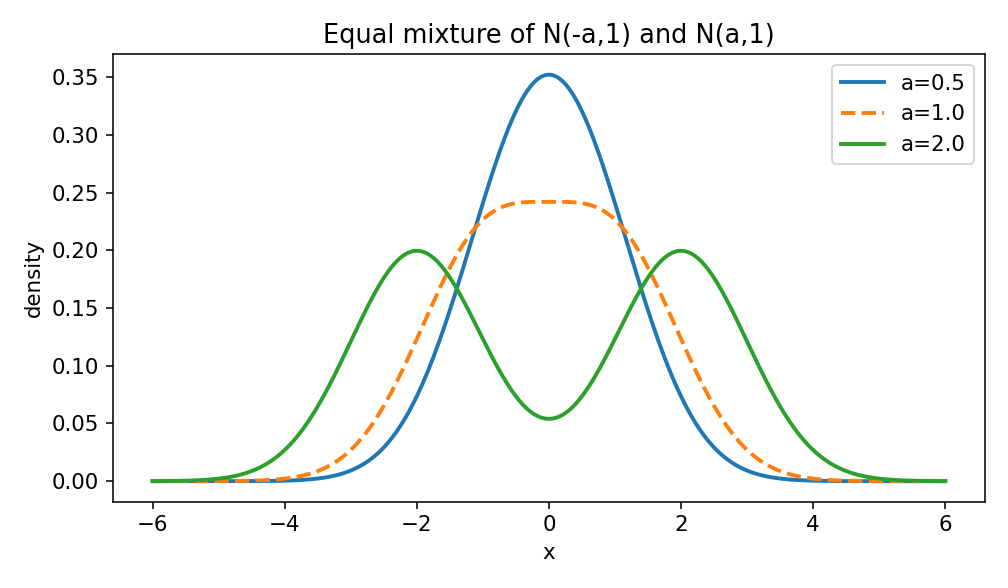
\includegraphics[width=0.72\textwidth]{HW1_figures/mixture_modes.png}
\caption{The mixture \(\tfrac12\N(-a,1)+\tfrac12\N(a,1)\). One peak for \(a\le 1\), two peaks for \(a>1\).}
\end{figure}

%----------------------------------------------------------------------
\section{Entropy, KL, and Jensen--Shannon}
\label{sec:info}
%----------------------------------------------------------------------

The slides define Kullback--Leibler divergence and then Jensen--Shannon divergence as its symmetric, smoothed version.

\begin{definition}[KL]
For discrete distributions,
\[
\KL(p\|q)=\E_{x\sim p}\Big[\log\frac{p(x)}{q(x)}\Big]
=\sum_x p(x)\log\frac{p(x)}{q(x)}.
\]
The continuous definition replaces the sum by an integral. In nats, \(\log=\ln\).
\end{definition}

Properties from the slides, all of which the homework uses:
\begin{itemize}
\item \(\KL(p\|q)\ge 0\), with equality if and only if \(p=q\).
\item \(\KL(p\|q)\ne\KL(q\|p)\) in general. KL is not a distance.
\item KL need not be finite, and it has no universal upper bound.
\item KL does not satisfy the triangle inequality.
\end{itemize}

\begin{definition}[Jensen--Shannon]
Let \(m=(p+q)/2\). Then
\[
\JS(p\|q)=\tfrac12\KL(p\|m)+\tfrac12\KL(q\|m).
\]
\end{definition}

Rewriting the definition in entropies, \(H(p)=-\sum p\log p\), gives
\[
\JS(p\|q)=H(m)-\tfrac12 H(p)-\tfrac12 H(q).
\]
Let \(Z\sim\Ber(1/2)\) and let \(X\mid Z=0\sim p\), \(X\mid Z=1\sim q\). Then \(X\sim m\) and \(\JS(p\|q)=I(Z;X)\). Mutual information is at most the entropy of \(Z\), so in nats
\[
0\le\JS(p\|q)\le\log 2.
\]
The lower bound holds when \(p=q\). The upper bound holds when \(p\) and \(q\) have disjoint supports. In bits the same bound reads \(0\le\JS\le 1\), and that form is sharp. The bound \(1\) in nats is true but not sharp: the sharp constant is \(\ln 2\).

\begin{toy}[Two Bernoulli divergences]
Let \(p=\Ber(0.9)\) and \(q=\Ber(0.1)\). Then
\begin{align*}
\KL(p\|q)&=0.9\log\frac{0.9}{0.1}+0.1\log\frac{0.1}{0.9}\approx 1.757,\\
\KL(q\|p)&=0.1\log\frac{0.1}{0.9}+0.9\log\frac{0.9}{0.1}\approx 1.757.
\end{align*}
These two happen to agree. Replace \(q\) by \(\Ber(0.01)\):
\[
\KL(p\|q)\approx 3.70,\qquad\KL(q\|p)\approx 0.36.
\]
The direction matters, which is Problem 2.4. The mixture \(m\) stays positive wherever \(p\) or \(q\) is positive, so \(\JS\) stays finite even in the limit where one Bernoulli parameter hits \(0\) and one of the two KLs diverges. That is Problem 2.3(a).
\end{toy}

\begin{figure}[ht]
\centering
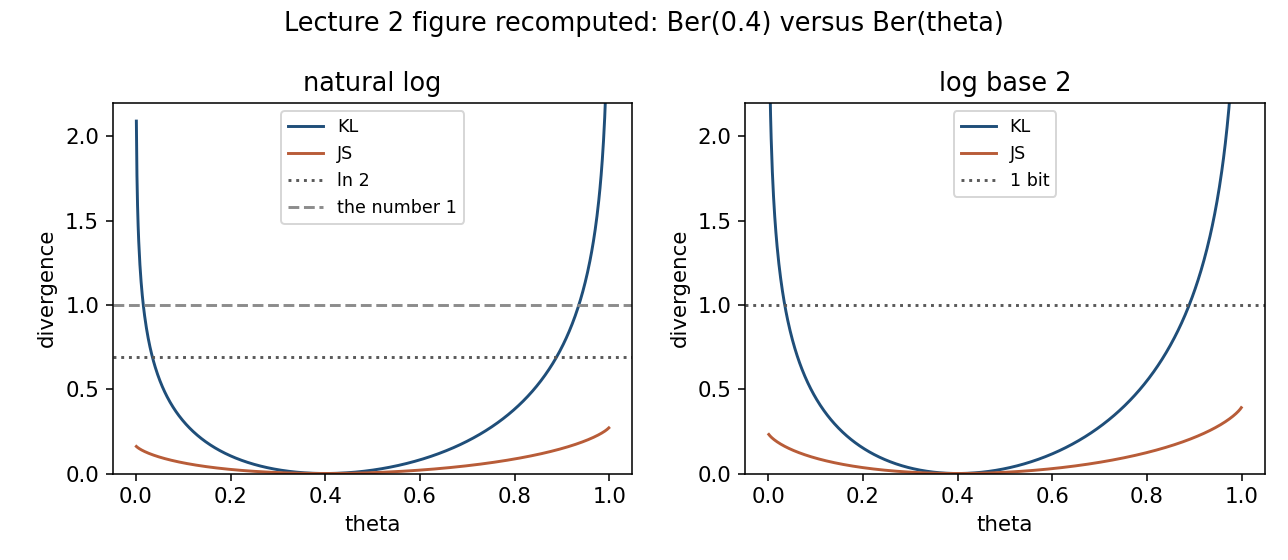
\includegraphics[width=0.78\textwidth]{HW1_figures/kl_js_bernoulli.png}
\caption{KL is asymmetric and unbounded. Jensen--Shannon on the same Bernoulli family stays inside \([0,\log 2]\).}
\end{figure}

\begin{result}[Gaussian KL]
For \(p_i=\N(\mu_i,\Sigma_i)\) with \(\Sigma_i\succ 0\),
\[
\KL(p_0\|p_1)
=\frac12\Big[
\tr(\Sigma_1^{-1}\Sigma_0)
+(\mu_0-\mu_1)^\top\Sigma_1^{-1}(\mu_0-\mu_1)
-d
+\log\frac{\det\Sigma_1}{\det\Sigma_0}
\Big].
\]
\end{result}

\begin{result}[Pythagoras for Gaussians]
Let \(p\) have mean \(\mu_p\) and covariance \(\Sigma_p\succ 0\), let \(g=\N(\mu_p,\Sigma_p)\), and let \(q\) be any Gaussian. Then
\[
\KL(p\|q)=\KL(p\|g)+\KL(g\|q).
\]
The best Gaussian approximation of \(p\), in the sense of \(\min_q\KL(p\|q)\), is \(g\) itself, and the minimum value is \(\KL(p\|g)=h(g)-h(p)\). Among all densities with a fixed mean and covariance, the Gaussian has the largest differential entropy.
\end{result}

The identity holds because \(\log(g/q)\) is a polynomial of degree at most \(2\), and \(p\) and \(g\) share moments of order \(0,1,2\), so they give that polynomial the same expectation.

%----------------------------------------------------------------------
\section{Autoregressive models}
\label{sec:ar}
%----------------------------------------------------------------------

\subsection{The factorization}

The chain rule says any positive density can be written
\[
p(x)=\prod_{d=1}^D p(x_d\mid x_{<d}).
\]
An autoregressive model picks a family for each factor. Training is maximum likelihood of those factors. Sampling is ancestral: draw \(x_1\), then \(x_2\) given \(x_1\), and so on. Density evaluation can be parallel in the coordinates once \(x\) is known, because every factor is a function of already-known numbers. Sampling cannot, because coordinate \(d\) is an input to every later factor.

For a nondegenerate Gaussian \(x\sim\N(0,\Sigma)\), each factor is itself Gaussian,
\[
x_d\mid x_{<d}\sim\N(w_d^\top x_{<d},\,\sigma_d^2),
\]
with \(w_d=\Sigma_{<d}^{-1}\Sigma_{<d,d}\) and \(\sigma_d^2\) the Schur complement. The conditional variance equals a ratio of principal minors,
\[
\sigma_d^2=\frac{\det\Sigma_{1:d}}{\det\Sigma_{1:d-1}},
\]
so \(\det\Sigma=\prod_d\sigma_d^2\). A strictly lower-triangular weight matrix has \(D(D-1)/2\) entries and there are \(D\) positive variances, which is exactly the number of free parameters in a covariance, \(D(D+1)/2\).

\begin{toy}[AR(1) on three coordinates]
Let \(\Sigma_{ij}=\rho^{|i-j|}\) with \(\rho=1/2\). This is a stationary AR(1) with innovation variance \(1-\rho^2=3/4\). The regressions are
\[
x_1\sim\N(0,1),\qquad
x_2\mid x_1\sim\N(\tfrac12 x_1,\tfrac34),\qquad
x_3\mid x_1,x_2\sim\N(\tfrac12 x_2,\tfrac34).
\]
Only the previous coordinate appears. Problem 1.5(a) is this calculation for the covariance written in the PDF, and Problem 1.5(b) shows that a different variable order fills in many more weights for the same joint law.
\end{toy}

\subsection{Markov tables}
\label{sec:markov}

Let each coordinate take values in \(\{1,\ldots,K\}\), and let \(c_i\) be the window of the \(m\) variables before position \(i\) (fewer at the start). An \emph{inhomogeneous} model of order \(m\) gives every position its own conditional table. A table with context length \(\ell\) has \(K^\ell(K-1)\) free numbers. Summing over positions,
\[
N_m^{\mathrm{nh}}
=(K^m-1)+(n-m)(K-1)K^m.
\]
A \emph{homogeneous} model uses one shared kernel after an arbitrary prefix of length \(m\), and has
\[
N_m^{\mathrm{h}}=K^{m+1}-1
\]
parameters. The difference is \((n-m-1)(K-1)K^m\). It is zero when \(n=m+1\): there is only one position that uses the kernel, so tying it to anything does not shrink the family. Both families are then the full simplex, of dimension \(K^n-1\).

\begin{toy}[Binary sequences of length 3, order 1]
Take \(K=2\), \(n=3\), \(m=1\).
\begin{itemize}
\item Inhomogeneous: position 1 has \(1\) free bit-probability, positions 2 and 3 each have a \(2\times 1\) conditional table, so \(1+2+2=5\) parameters. The formula gives \((2-1)+(3-1)\cdot 1\cdot 2=5\).
\item Homogeneous: a prefix bit and one shared \(2\times 1\) kernel, so \(1+2=3\) parameters. The formula gives \(2^{2}-1=3\).
\end{itemize}
The two missing parameters are exactly the freedom to let position 3 use a different kernel from position 2.
\end{toy}

%----------------------------------------------------------------------
\section{Bayesian networks and valid orders}
\label{sec:bn}
%----------------------------------------------------------------------

A directed acyclic graph on variables \(v\) defines
\[
p(x)=\prod_v p(x_v\mid x_{\pa(v)}).
\]
Acyclicity is what makes this a probability distribution. Sum the variables in a topological order, child after all of its parents. Each conditional sums to \(1\), so the product sums to \(1\). A directed cycle has no such order, and the same formal product need not sum to \(1\).

For binary variables a conditional with \(k\) parents has \(2^k\) free parameters (one probability for each parent configuration).

Figure~1 of the homework, read from the arrowheads, has the edges
\[
B\to E,\; B\to G,\; E\to G,\qquad
A\to C,\; A\to D,\; D\to F,\; C\to F.
\]
The parents are \(\pa(C)=\{A\}\), \(\pa(D)=\{A\}\), \(\pa(E)=\{B\}\), \(\pa(F)=\{C,D\}\), \(\pa(G)=\{B,E\}\).

\begin{figure}[ht]
\centering
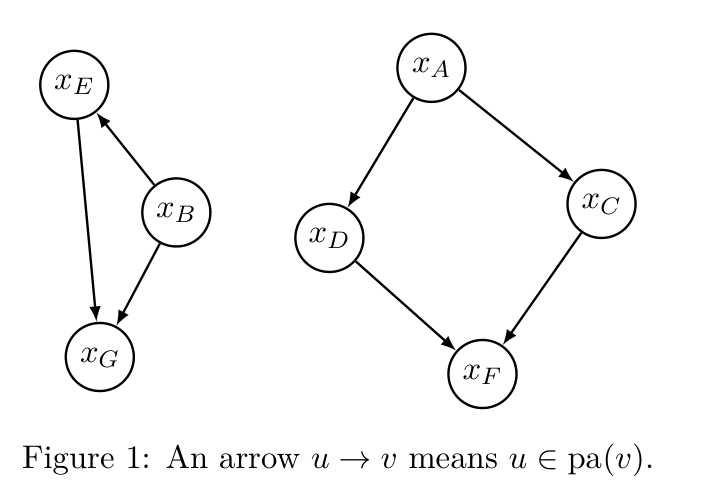
\includegraphics[width=0.55\textwidth]{HW1_figures/figure1_from_pdf.png}
\caption{Figure 1 of the homework. Edges point \(B\to E\to G\), \(B\to G\), and \(A\to C\), \(A\to D\to F\), \(C\to F\).}
\end{figure}

A valid ordering is a topological ordering. On \(\{B,E,G\}\) the only order is \(B,E,G\). On \(\{A,C,D,F\}\) the node \(A\) is first, \(F\) is last, and \(\{C,D\}\) can be swapped, which is \(2\) orders. Interleaving a block of \(3\) with a block of \(4\) can be done in \(\binom{7}{3}\) ways, so there are
\[
\binom{7}{3}\cdot 1\cdot 2=70
\]
valid orders, and \(70/7!=1/72\).

\begin{toy}[A two-node cycle does not normalize]
The smallest version of Problem 3.3(c): put \(q(x,y)=p(x\mid y)\,p(y\mid x)\) with
\[
p(x=1\mid y)=\theta_y,\qquad p(y=1\mid x)=\varphi_x.
\]
Summing the four atoms leaves \(Z=1+(\theta_0-\theta_1)(\varphi_0-\varphi_1)\), which equals \(1\) for every parameter only if at least one conditional ignores its parent. A cycle is not a free modelling choice. It changes the normalizer.
\end{toy}

%----------------------------------------------------------------------
\section{FVSBN, NADE, and MADE}
\label{sec:nade}
%----------------------------------------------------------------------

All three models below are autoregressive factorizations of a binary vector \(x\in\{0,1\}^D\),
\[
p(x)=\prod_{d=1}^D p(x_d\mid x_{<d}),\qquad
p(x_d\mid x_{<d})=\Ber\big(\sigma(z_d)\big),
\]
with \(\sigma(z)=1/(1+e^{-z})\). They differ in how the logit \(z_d\) may depend on the past.

\subsection{FVSBN}

A fully visible sigmoid belief network uses an affine logit,
\[
z_1=b_1,\qquad z_d=b_d+w_d^\top x_{<d}\ (d\ge 2).
\]
Parameter count: \(D+\sum_{d=2}^D(d-1)=D(D+1)/2\). At \(D=784\) this is \(307720\), of which the multiplications that form \(\log p(x)\) use \(D(D-1)/2=306936\).

An affine function on the cube is determined by its values: the bias is the value at \(0\), and each weight is a finite difference along one axis. So different parameters give different distributions. The family has dimension \(D(D+1)/2\). The simplex of all positive pmfs on \(\{0,1\}^D\) has dimension \(2^D-1\). These meet at \(D=1\) and \(D=2\) only.

The obstruction is an interaction. An affine logit has zero second differences,
\[
\ell(1,1)-\ell(1,0)-\ell(0,1)+\ell(0,0)=0.
\]
Parity, \(p(x)\propto\theta\) on odd strings and \(1-\theta\) on even strings, has second difference \(4\log(\theta/(1-\theta))\ne 0\). No FVSBN represents it.

\subsection{NADE}

NADE shares one hidden state across the conditionals. With \(a_1\) unused and
\[
a_d=c+\sum_{k<d}W_{:,k}x_k,\qquad h_d=\phi(a_d),\qquad z_d=v_d^\top h_d+b_d
\]
for \(d\ge 2\), and \(z_1=b_1\), the parameter count is
\[
D_h(D-1)+D_h+(D-1)D_h+D=D_h(2D-1)+D.
\]
NADE is smaller than an FVSBN when \(D_h<D(D-1)/(2(2D-1))\). For \(D=784\) the largest such integer is \(D_h=195\).

The recursion \(a_{d+1}=a_d+W_{:,d}x_d\) evaluates every hidden state in \(2(D-1)D_h\) multiplications. At \(D=784\), \(D_h=500\) that is \(783000\), against \(153859500\) if each \(a_d\) is recomputed from scratch, and against \(306936\) for the FVSBN. The recursion does not let you sample in parallel. Coordinate \(d\) is still unknown until it has been drawn.

The Bernoulli negative log-likelihood in the logit has derivative \(\delta_d=\sigma(z_d)-x_d\). Backpropagation through the shared \(a_d\) gives
\begin{align*}
\frac{\partial L}{\partial b_d}&=\delta_d, &
\frac{\partial L}{\partial v_d}&=\delta_d h_d, &
\frac{\partial L}{\partial h_d}&=\delta_d v_d,\\
\frac{\partial L}{\partial a_d}&=\phi'(a_d)\odot(\delta_d v_d), &
\frac{\partial L}{\partial c}&=\sum_{d\ge 2}\frac{\partial L}{\partial a_d}, &
\frac{\partial L}{\partial W_{:,k}}&=x_k\sum_{d>k}\frac{\partial L}{\partial a_d}.
\end{align*}
The sums telescope. One forward pass and one backward accumulation compute every column gradient.

For \(\phi=\tanh\), flipping the sign of hidden unit \(j\) in \(c\), in row \(j\) of \(W\), and in coordinate \(j\) of every \(v_d\) leaves \(v_d^\top h_d\) unchanged, because \(\tanh\) is odd. Permuting the hidden coordinates does the same. A generic parameter therefore has at least \(D_h!\,2^{D_h}\) preimages.

\subsection{MADE masks}

MADE enforces the same dependence with multiplicative masks. Input \(i\) has degree \(m^0(i)\in\{1,\ldots,D\}\), a permutation of the coordinates. Hidden unit \(k\) has degree \(m^1(k)\in\{1,\ldots,D-1\}\). Output \(d\) has degree \(m^0(d)\). The masks are
\[
[M^W]_{ki}=\mathbf{1}\{m^1(k)\ge m^0(i)\},\qquad
[M^V]_{dk}=\mathbf{1}\{m^0(d)>m^1(k)\}.
\]
A hidden unit may read an input of equal or smaller degree. An output may read a hidden unit only of \emph{strictly} smaller degree. The strictness is what stops coordinate \(d\) from seeing itself.

\begin{figure}[ht]
\centering
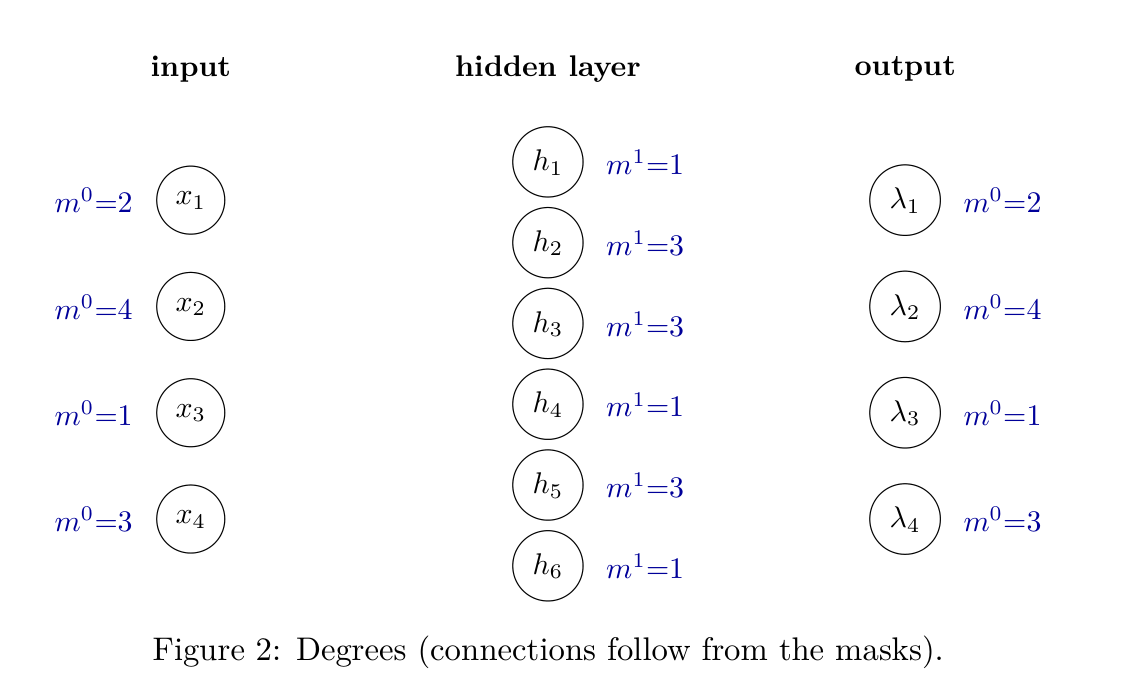
\includegraphics[width=0.85\textwidth]{HW1_figures/figure2_from_pdf.png}
\caption{Figure 2. Degrees: \(x_1\) and \(\lambda_1\) have \(m^0=2\); \(x_2,\lambda_2\) have \(m^0=4\); \(x_3,\lambda_3\) have \(m^0=1\); \(x_4,\lambda_4\) have \(m^0=3\). Hidden degrees: \(h_1,h_4,h_6\) have \(m^1=1\), and \(h_2,h_3,h_5\) have \(m^1=3\).}
\end{figure}

The induced order is increasing degree: \(x_3,x_1,x_4,x_2\). Output \(\lambda_d\) can depend only on inputs of degree strictly less than \(m^0(d)\). In the figure, \(\lambda_4\) is allowed by the order to see \(x_1\), but no hidden unit has degree \(2\), which is the only degree that both sees \(x_1\) and is allowed to write to \(\lambda_4\). One hidden unit of each degree \(1,2,\ldots,D-1\) restores every dependence the order allows, so the smallest such width is \(H=D-1\). That restores connectivity, not the ability to represent an arbitrary conditional table.

If the output rule is weakened to a non-strict inequality, a hidden unit of degree \(m^0(d)\) can connect to \(\lambda_d\) and can also read \(x_d\). Then \(\lambda_d\) depends on \(x_d\), and summing the Bernoulli factor in \(x_d\) need not give \(1\).

\begin{toy}[Masks on three bits]
Take \(D=3\), degrees \(m^0=(1,2,3)\) on \((x_1,x_2,x_3)\), and two hidden units of degrees \(1\) and \(2\). Then
\[
M^W=\begin{pmatrix}1&0&0\\1&1&0\end{pmatrix},\qquad
M^V=\begin{pmatrix}0&0\\1&0\\1&1\end{pmatrix}.
\]
Output \(1\) sees nothing. Output \(2\) sees only the hidden unit of degree \(1\), which sees only \(x_1\). Output \(3\) sees both hidden units, hence \(x_1\) and \(x_2\), and not \(x_3\). Drop the hidden unit of degree \(1\) and the edge \(x_1\to\lambda_2\) disappears, exactly as \(x_1\to\lambda_4\) disappears in Figure~2.
\end{toy}

%----------------------------------------------------------------------
\section{Real-valued autoregression}
\label{sec:real}
%----------------------------------------------------------------------

Real NADE replaces the Bernoulli factor by a Gaussian whose mean and log-variance are both read from the hidden state. The homework writes the variance as \(e^{s_d}\), with a bias \(e_d\) in the log-variance (the slides sometimes call this bias \(d_d\); it is the same parameter):
\[
p(x_d\mid x_{<d})=\N(x_d\mid\mu_d,e^{s_d}),\qquad
\mu_d=v_d^\top h_d+b_d,\qquad
s_d=u_d^\top h_d+e_d.
\]
The negative log-density on one coordinate is
\[
\ell(x;\mu,s)=\tfrac12\log(2\pi)+\tfrac s2+\frac{(x-\mu)^2}{2e^{s}}.
\]
Differentiating,
\[
\delta^\mu:=\frac{\partial\ell}{\partial\mu}=-(x-\mu)e^{-s},\qquad
\delta^s:=\frac{\partial\ell}{\partial s}=\tfrac12-\tfrac12(x-\mu)^2 e^{-s}.
\]
The Hessian in \((\mu,s)\) is
\[
\nabla^2\ell
=\begin{pmatrix}
e^{-s} & (x-\mu)e^{-s}\\
(x-\mu)e^{-s} & \tfrac12(x-\mu)^2 e^{-s}
\end{pmatrix},
\]
with determinant \(-\tfrac12(x-\mu)^2 e^{-2s}\). Whenever \(x\ne\mu\) the Hessian is indefinite, so \(\ell\) is not jointly convex in \((\mu,s)\). It is convex in each argument separately. In the natural parameters \(\eta_1=\mu e^{-s}\) and \(\eta_2=-\tfrac12 e^{-s}\) it is strictly convex, because the log-partition function of that exponential family is strictly convex.

A single Gaussian fitted to one point is unbounded: put the mean on the point and send the variance to \(0\). The log-density goes to \(+\infty\). Two or more distinct points stop that escape, because a Gaussian has only one variance. A mixture of two Gaussians opens the escape again: one component collapses onto one point, and another component keeps the remaining points at a finite density.

\begin{toy}[A one-point Gaussian]
One observation \(x=0\). Set \(\mu=0\). Then \(\ell(0;0,s)=s/2+\tfrac12\log(2\pi)\), which tends to \(-\infty\) as \(s\to-\infty\). The likelihood tends to \(+\infty\). Add a second observation at \(1\). The profile over the variance is minimized at the empirical second moment and the negative log-likelihood stays finite. This is the difference between Problem 5.3 and Problem 5.3 with \(N\ge 2\).
\end{toy}

%----------------------------------------------------------------------
\section{Generative and discriminative classifiers}
\label{sec:disc}
%----------------------------------------------------------------------

A generative classifier models \(p(y)\,p(x\mid y)\) and applies Bayes' rule. A discriminative classifier models \(p(y\mid x)\) directly. For two classes, \(p(y=1)=\pi\) and \(x\mid y=c\sim\N(\mu_c,\Sigma_c)\),
\[
p(y=1\mid x)=\sigma(a(x)),\qquad
a(x)=\log\frac{\pi}{1-\pi}+\log\N(x\mid\mu_1,\Sigma_1)-\log\N(x\mid\mu_0,\Sigma_0).
\]
If \(\Sigma_0=\Sigma_1=\Sigma\), the quadratic terms cancel and \(a(x)=w^\top x+b\) with
\[
w=\Sigma^{-1}(\mu_1-\mu_0),\qquad
b=-w^\top\bar\mu+\log\frac{\pi}{1-\pi},
\]
where \(\bar\mu=\tfrac12(\mu_0+\mu_1)\). Logistic regression is exactly this functional form, with \((w,b)\) free. Many generative parameters produce the same \((w,b)\): any covariance and any midpoint, with the class gap and the prior then fixed by \(w\) and \(b\). That fiber has dimension \(D(D+3)/2\).

If the covariances differ, \(a(x)\) is a genuine quadratic polynomial. Logistic regression cannot represent it.

\begin{toy}[One-dimensional shared variance]
Let \(\pi=1/2\), \(\mu_0=-1\), \(\mu_1=1\), \(\Sigma=1\). Then \(w=2\) and \(b=0\), so \(p(y=1\mid x)=\sigma(2x)\). The decision boundary is \(x=0\), halfway between the class means. Masking is vacuous in one dimension. In several dimensions, replacing a missing block by the midpoint \(\bar\mu_M\) does \emph{not} reproduce the Bayes rule that simply ignores those coordinates. Problem 6.2 is that comparison.
\end{toy}

\newpage
%----------------------------------------------------------------------
\section{Problem 1, step by step}
%----------------------------------------------------------------------

Throughout, \(x\sim\N(\mu,\Sigma)\) means the mgf identity in the PDF, and jointly Gaussian vectors are independent if and only if they are uncorrelated.

\subsection*{1.1 Law of \texorpdfstring{\(y=Ax+b\)}{y = Ax + b}}
\addcontentsline{toc}{subsection}{1.1 Law of y = Ax + b}

Compute the mgf of \(y=Ax+b\):
\[
\E[e^{s^\top y}]
=e^{s^\top b}\exp\big((A^\top s)^\top\mu+\tfrac12(A^\top s)^\top\Sigma A^\top s\big).
\]
This is the mgf of
\[
\boxed{y\sim\N(A\mu+b,\,A\Sigma A^\top)}.
\]

\subsection*{1.1(a) Scalar combinations, and a bound on correlation}
\addcontentsline{toc}{subsection}{1.1(a) Scalar combinations, and a bound on correlation}

Let \((x,y)\) be jointly Gaussian with cross-covariance \(C\). Apply 1.1 to the row \((a,b)\):
\[
z=ax+by\sim\N\big(a\mu_x+b\mu_y,\;
a^2\Sigma_x+b^2\Sigma_y+ab\,C+ab\,C^\top\big).
\]
The covariance of \(z\) is singular when this matrix is singular. Two cases the problem asks you to look at:
\begin{itemize}
\item If \(x\perp y\), then \(C=0\). For scalars, \(\Var(z)=a^2\Var(x)+b^2\Var(y)\), which is singular only when \(z\) is almost surely constant.
\item If \(y=x\), then \(z=(a+b)x\), which is supported on a line. In several dimensions the covariance has rank at most \(\operatorname{rank}\Cov(x)\).
\end{itemize}
In dimension one, with correlation \(\rho\),
\[
\Var(z)=a^2\sigma_x^2+b^2\sigma_y^2+2ab\rho\,\sigma_x\sigma_y.
\]
This quadratic form in \((a\sigma_x,b\sigma_y)\) is nonnegative for every \((a,b)\) if and only if \(|\rho|\le 1\). Equality \(|\rho|=1\) is attained when \(y\) is an affine function of \(x\), because that is when the \(2\times 2\) covariance is singular and nonzero.

\subsection*{1.1(b) A tall thin linear image}
\addcontentsline{toc}{subsection}{1.1(b) A tall thin linear image}

Let \(x\sim\N(0,I_d)\) and let \(A\in\R^{m\times d}\) with \(m>d\) and full column rank. Then \(\Cov(Ax)=AA^\top\) has rank \(d<m\), so \(Ax\) has no density on \(\R^m\).

Write the thin QR factorization \(A=QR\), with \(Q\in\R^{m\times d}\) having orthonormal columns and \(R\in\R^{d\times d}\) invertible. Then \(Ax=Q(Rx)\) and
\[
Rx\sim\N(0,RR^\top),
\]
which \emph{does} have a density on \(\R^d\), because \(RR^\top\succ 0\). The random vector \(Ax\) is that nondegenerate Gaussian, embedded by \(Q\).

The squared norm has expectation
\[
\E[\lVert Ax\rVert^2]
=\E[x^\top A^\top A x]
=\tr(A^\top A)
=\lVert A\rVert_F^2.
\]
The same number is \(\tr(AA^\top)\), and also \(\E[\lVert Rx\rVert^2]\) because \(Q\) preserves Euclidean norm. Both routes agree.

\subsection*{1.2 Product identity}
\addcontentsline{toc}{subsection}{1.2 Product identity}

Match quadratic and linear terms in the exponent, as in the toy of \S\ref{sec:gauss}. The result is
\[
\boxed{C=(A^{-1}+B^{-1})^{-1}=A(A+B)^{-1}B,\quad
c=C(A^{-1}a+B^{-1}b),\quad
Z=\N(a\mid b,A+B)}.
\]
The two formulas for \(C\) are the same matrix. The form that inverts only \(A+B\) is the one used when \(A^{-1}\) and \(B^{-1}\) are inconvenient but \(A+B\) is not.

\subsection*{1.2(a) Gaussian posterior, marginal, MLE, MAP}
\addcontentsline{toc}{subsection}{1.2(a) Gaussian posterior, marginal, MLE, MAP}

Prior \(\theta\sim\N(m_0,s_0^2)\). Likelihood: \(x_i\mid\theta\) i.i.d.\ \(\N(\theta,s^2)\). The product identity, applied \(n\) times, gives the posterior
\[
\theta\mid x_{1:n}\sim\N(m_n,s_n^2),
\]
\[
s_n^2=\frac{s_0^2 s^2}{s^2+n s_0^2},\qquad
m_n=\frac{s^2 m_0+n s_0^2\bar x}{s^2+n s_0^2}.
\]
The joint law of \((x_1,\ldots,x_n)\) is Gaussian. Its mean is \(m_0\mathbf{1}\). Its covariance is \(s^2 I+s_0^2\mathbf{1}\mathbf{1}^\top\), because \(x_i=m_0+\eta+\varepsilon_i\) with \(\eta\sim\N(0,s_0^2)\) the shared prior draw.

The likelihood in \(\theta\) is maximized at the sample mean: \(\hat\theta_{\mathrm{MLE}}=\bar x\). The posterior mode is the posterior mean, since the posterior is Gaussian:
\[
\hat\theta_{\mathrm{MAP}}=m_n
=(1-\alpha)m_0+\alpha\bar x,
\qquad
\alpha=\frac{n s_0^2}{s^2+n s_0^2}.
\]
As \(n\to\infty\), \(\alpha\to 1\) and \(s_n^2\to 0\), so the MAP collapses to the MLE. As \(s_0\to\infty\), the prior flattens, \(\alpha\to 1\), and again the MAP tends to the MLE.

\subsection*{1.3 Conditional law}
\addcontentsline{toc}{subsection}{1.3 Conditional law}

Use the residual argument of \S\ref{sec:gauss}. With \(K=\Sigma_{yx}\Sigma_{xx}^{-1}\),
\[
\boxed{y\mid x=x_0\sim\N\big(\mu_y+K(x_0-\mu_x),\;
\Sigma_{yy}-K\Sigma_{xy}\big)}.
\]
The covariance does not depend on \(x_0\). It equals \(\Sigma_{yy}\) if and only if \(\Sigma_{yx}=0\).

\subsection*{1.3(a) Linear-Gaussian model, two forms of the posterior}
\addcontentsline{toc}{subsection}{1.3(a) Linear-Gaussian model, two forms of the posterior}

Now \(x\sim\N(\mu,\Sigma)\) and \(y\mid x\sim\N(Ax+b,S)\) with \(S\succ 0\).

The joint of \((x,y)\) is Gaussian, with mean \((\mu,\,A\mu+b)\) and covariance
\[
\begin{pmatrix}
\Sigma & \Sigma A^\top\\
A\Sigma & S+A\Sigma A^\top
\end{pmatrix}.
\]
The marginal of \(y\) is the bottom-right block: \(y\sim\N(A\mu+b,\,S+A\Sigma A^\top)\).

The posterior covariance of \(x\) given \(y\) is the conditional covariance from 1.3, which the matrix inversion lemma rewrites without a Schur complement in \(\Sigma\):
\[
\Cov(x\mid y)
=(\Sigma^{-1}+A^\top S^{-1}A)^{-1}
=\Sigma-\Sigma A^\top(S+A\Sigma A^\top)^{-1}A\Sigma.
\]
The two expressions agree by the Woodbury identity. The posterior mean is
\[
\E[x\mid y]
=\mu+\Cov(x\mid y)\,A^\top S^{-1}\big(y-(A\mu+b)\big).
\]
The matrix multiplying the innovation \(y-(A\mu+b)\) is the Kalman gain. It converts a residual in observation space into a correction in \(x\)-space. The second form of the gain, \(\Sigma A^\top(S+A\Sigma A^\top)^{-1}\), inverts only the marginal covariance of \(y\).

\subsection*{1.4 Mixture moments}
\addcontentsline{toc}{subsection}{1.4 Mixture moments}

Condition on the component, as in \S\ref{sec:gauss}:
\[
\E[x]=\sum_k\pi_k\mu_k,
\]
\[
\E[xx^\top]=\sum_k\pi_k(\Sigma_k+\mu_k\mu_k^\top),
\]
and the covariance splits into \(\sum_k\pi_k\Sigma_k\) (within) plus \(\sum_k\pi_k(\mu_k-\mu)(\mu_k-\mu)^\top\) (between).

\subsection*{1.4(a) Two components on the line}
\addcontentsline{toc}{subsection}{1.4(a) Two components on the line}

Let \(p=\tfrac12\N(-a,1)+\tfrac12\N(a,1)\) with \(a>0\).
\begin{itemize}
\item Mean: the two centers cancel, so \(\E[x]=0\).
\item Variance: within contribution \(1\), between contribution \(a^2\), so \(\Var(x)=1+a^2\).
\item Fourth moment: a \(\N(a,1)\) random variable has \(\E[Z^4]=a^4+6a^2+3\), and the same value at \(-a\). Excess kurtosis:
\[
\frac{a^4+6a^2+3}{(1+a^2)^2}-3=\frac{-2a^4}{(1+a^2)^2}<0.
\]
A Gaussian would give \(0\), so \(p\) is not Gaussian. Its mgf is \(\cosh(at)\,e^{t^2/2}\), which is not a Gaussian mgf.
\end{itemize}

Modes. The unnormalized density \(h(x)=e^{-(x+a)^2/2}+e^{-(x-a)^2/2}\) has no critical point outside \([-a,a]\). Inside,
\[
h'(x)=0\iff\frac{a+x}{a-x}=e^{2ax}.
\]
Set \(k(x)=\log(a+x)-\log(a-x)-2ax\). Then \(k(0)=0\) and
\[
k'(x)=2a\frac{x^2-(a^2-1)}{a^2-x^2},\qquad
h''(0)=2(a^2-1)e^{-a^2/2}.
\]
\begin{itemize}
\item If \(a<1\), then \(k'>0\) on \((0,a)\), so \(x=0\) is the only root, and \(h''(0)<0\). One mode.
\item If \(a=1\), the only root is still \(x=0\), and the next term of \(h''\) shows it is a strict local maximum. One mode.
\item If \(a>1\), then \(k\) has one positive root, hence three real critical points, and \(h''(0)>0\), so \(x=0\) is a local minimum. Two modes.
\end{itemize}
So \(p\) has two modes if and only if \(a>1\).

\subsection*{1.4(b) Gaussian KL, Pythagoras, maximum entropy}
\addcontentsline{toc}{subsection}{1.4(b) Gaussian KL, Pythagoras, maximum entropy}

(i) Expand \(-\E_{p_0}\log p_1\) and subtract the entropy of \(p_0\). The quadratic form contributes a trace plus a mean shift, and the normalizers contribute the log-determinant. The result is the Gaussian KL stated in \S\ref{sec:info}.

(ii) Let \(g=\N(\mu_p,\Sigma_p)\) and let \(q\) be any Gaussian. Then \(\log(g/q)\) has degree at most \(2\), so
\[
\KL(p\|q)-\KL(p\|g)=\E_p\log\frac{g}{q}=\E_g\log\frac{g}{q}=\KL(g\|q).
\]
Hence \(\KL(p\|q)=\KL(p\|g)+\KL(g\|q)\). The second term is nonnegative and zero only at \(q=g\). The best Gaussian is \(g\), and
\[
\min_q\KL(p\|q)=\KL(p\|g)=h(g)-h(p).
\]
Applied to the mixture of 1.4(a): that mixture has mean \(0\) and variance \(1+a^2\), so its best Gaussian approximation is \(\N(0,1+a^2)\), and the minimal KL equals the entropy gap. Among densities with those two moments the Gaussian maximizes \(h\), because the gap is nonnegative.

\subsection*{1.5 Autoregressive factorization of a Gaussian}
\addcontentsline{toc}{subsection}{1.5 Autoregressive factorization of a Gaussian}

By 1.3 applied to the last coordinate,
\[
w_d=\Sigma_{<d}^{-1}\Sigma_{<d,d},\qquad
\sigma_d^2=\Sigma_{dd}-\Sigma_{d,<d}\Sigma_{<d}^{-1}\Sigma_{<d,d},
\]
and \(x_d\mid x_{<d}\sim\N(w_d^\top x_{<d},\sigma_d^2)\), with \(\sigma_1^2=\Sigma_{11}\). The conditional law is unique, so the factorization is unique. The Schur complement satisfies \(\sigma_d^2=\det\Sigma_{1:d}/\det\Sigma_{1:d-1}\), hence \(\det\Sigma=\prod_d\sigma_d^2\).

A strictly lower-triangular \(W\) together with \(D\) positive conditional variances has \(D(D+1)/2\) free parameters, matching \(\Sigma\succ 0\). Conversely, \(x_d=w_d^\top x_{<d}+\varepsilon_d\) with independent \(\varepsilon_d\sim\N(0,\sigma_d^2)\) is \(x=(I-W)^{-1}\varepsilon\), and
\[
x\sim\N\big(0,\,(I-W)^{-1}\Delta(I-W)^{-\top}\big),
\qquad\Delta=\operatorname{diag}(\sigma_d^2).
\]

\subsection*{1.5(a) The AR(1) covariance}
\addcontentsline{toc}{subsection}{1.5(a) The AR(1) covariance}

The covariance in the PDF is the stationary AR(1) covariance
\[
\Sigma_{ij}=\frac{\sigma^2}{1-\rho^2}\rho^{|i-j|},\qquad|\rho|<1.
\]
It is produced by
\[
x_1\sim\N\Big(0,\frac{\sigma^2}{1-\rho^2}\Big),\qquad
x_d=\rho x_{d-1}+\varepsilon_d,\quad\varepsilon_d\sim\N(0,\sigma^2).
\]
Reading the regression off \(\Sigma\): \(\sigma_1^2=\sigma^2/(1-\rho^2)\), and for \(d\ge 2\) the weight vector \(w_d\) has a single nonzero entry \(\rho\) in the coordinate of \(x_{d-1}\), with conditional variance \(\sigma_d^2=\sigma^2\). The normal equations hold because a column of this Toeplitz matrix, scaled by \(\rho\), reproduces the next column.

\subsection*{1.5(b) Hub and leaves}
\addcontentsline{toc}{subsection}{1.5(b) Hub and leaves}

Model: \(x_1\sim\N(0,1)\) and \(x_j=\beta x_1+\varepsilon_j\) for \(j\ge 2\), with \(\varepsilon_j\sim\N(0,s^2)\) independent and \(\beta\ne 0\). Then
\[
\Sigma
=\begin{pmatrix}
1 & \beta\mathbf{1}^\top\\
\beta\mathbf{1} & s^2 I+\beta^2\mathbf{1}\mathbf{1}^\top
\end{pmatrix}.
\]

Order \((1,\ldots,D)\). The hub is first, \(\sigma_1^2=1\), and each leaf satisfies \(w_j=\beta e_1\), \(\sigma_j^2=s^2\). There are \(D-1\) nonzero weights, and \(\prod_d\sigma_d^2=(s^2)^{D-1}\).

Order \((D,\ldots,1)\). At position \(m+1\), a new leaf is conditioned on \(m\) earlier leaves. The constant weight
\[
c=\frac{\beta^2}{s^2+m\beta^2}
\]
solves the normal equations, and
\[
\sigma^2=\frac{s^2\big(s^2+(m+1)\beta^2\big)}{s^2+m\beta^2}.
\]
The hub, placed last, has weight \(\beta/(s^2+(D-1)\beta^2)\) on every leaf and conditional variance \(s^2/(s^2+(D-1)\beta^2)\). Nonzero weights: \(\sum_{m=1}^{D-2}m+(D-1)=D(D-1)/2\).

The product of conditional variances equals \(\det\Sigma\) in every order, so both orders give \((s^2)^{D-1}\).

The pair \((W,\Delta)\) is unique for a fixed order. In the leaf-first order, the row in position \(m+1\) has \(m\) nonzeros. For \(D\ge 3\) and \(m\ge 2\) that is more than one nonzero, while every row of the hub-first factorization has at most one. A model restricted to the hub-first sparsity pattern cannot represent this law in the reversed order.

\subsection*{1.5(c) A conditional variance that depends on the value}
\addcontentsline{toc}{subsection}{1.5(c) A conditional variance that depends on the value}

No. By 1.3, a nondegenerate joint Gaussian has a conditional covariance that does not depend on the conditioning value. Here \(\Var(x_2\mid x_1)=e^{ux_1}\) depends on \(x_1\) because \(u\ne 0\).

\newpage
%----------------------------------------------------------------------
\section{Problem 2, step by step}
%----------------------------------------------------------------------

\subsection*{2.1 Monte Carlo}
\addcontentsline{toc}{subsection}{2.1 Monte Carlo}

Let \(x_n\) be i.i.d.\ from \(p\) and \(f_N=N^{-1}\sum_n f(x_n)\). If \(\E_p|f|<\infty\), then \(\E[f_N]=\E_p[f]\): the estimator is unbiased. If \(\Var_p(f)=\sigma_f^2<\infty\), independence gives \(\Var(f_N)=\sigma_f^2/N\). Chebyshev is
\[
\Pr\big(|f_N-\E f|\ge\varepsilon\big)\le\frac{\sigma_f^2}{N\varepsilon^2}.
\]
This tends to \(0\), which is the weak law, and it forces \(N\ge\sigma_f^2/(\delta\varepsilon^2)\) to reach deviation \(\varepsilon\) with probability at most \(\delta\).

\subsection*{2.1(a) Three sample sizes for the same tail}
\addcontentsline{toc}{subsection}{2.1(a) Three sample sizes for the same tail}

From the toy in \S\ref{sec:moments}: \(\E[f]=4\), \(\Var(f)=32\), and \(f_N=(4/N)\chi^2_N\). The event \(|f_N-4|\ge 1/2\) is a relative deviation \(t=1/8\) of the chi-squared variable.

\begin{enumerate}
\item Chebyshev. \(\Var(f_N)=32/N\), so the probability is at most \(128/N\). This is at most \(0.05\) once \(N\ge 2560\). The bound is a theorem. It is guaranteed.
\item CLT. Ask that \((1/2)/\sqrt{32/N}\ge 1.96\). This gives \(N\ge 492\). The chi-squared law is skewed, so the normal tail is not an upper bound at finite \(N\). This number is not guaranteed.
\item Chernoff. The mgf of \(\chi^2_N\) yields, for \(t\in(0,1)\),
\begin{align*}
\Pr(\chi^2_N\ge N(1+t))&\le\big((1+t)e^{-t}\big)^{N/2},\\
\Pr(\chi^2_N\le N(1-t))&\le\big((1-t)e^{t}\big)^{N/2}.
\end{align*}
At \(t=1/8\) the sum of the two bounds drops to \(0.05\) or below at \(N=950\) (the bound is \(0.04983\) at \(950\) and \(0.05002\) at \(949\)). Nearest \(50\) is \(950\). This \(N\) is guaranteed, because it comes from the mgf.
\end{enumerate}
Chebyshev uses only the variance, so it is loose. Chernoff uses the mgf and is tighter, but it is still a bound. The CLT is the most optimistic of the three because it is not a finite-sample guarantee.

\begin{figure}[ht]
\centering
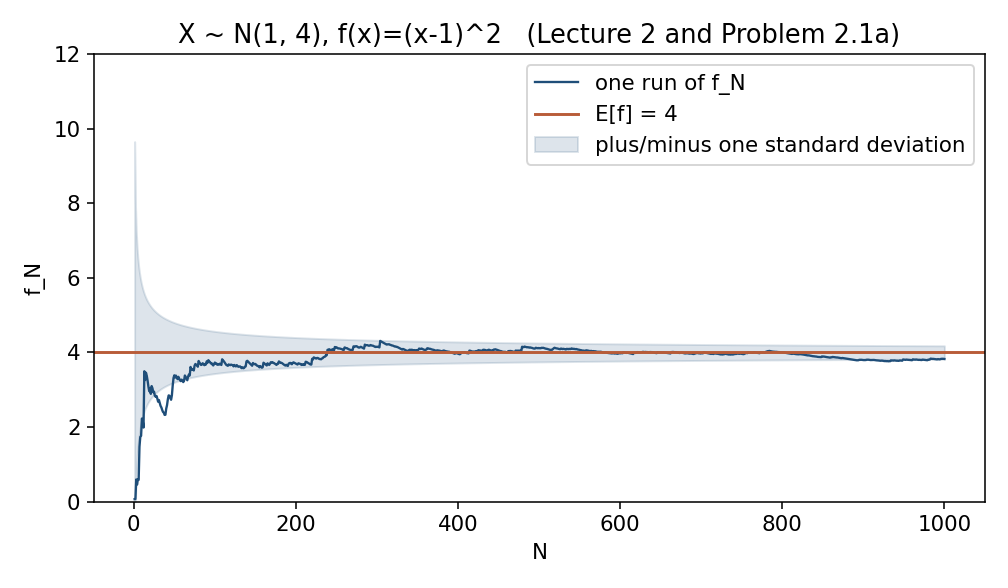
\includegraphics[width=0.72\textwidth]{HW1_figures/monte_carlo.png}
\caption{The same deviation, three ways. Chebyshev at \(2560\), Chernoff at \(950\), and a CLT suggestion near \(492\) that is not guaranteed.}
\end{figure}

\subsection*{2.1(b) Importance sampling}
\addcontentsline{toc}{subsection}{2.1(b) Importance sampling}

Draw \(x_n\sim q=\N(0,s^2)\) and set \(\hat I_N=N^{-1}\sum_n x_n^2\,p(x_n)/q(x_n)\), with \(p=\N(0,1)\) and \(f(x)=x^2\). Since \(q>0\) everywhere,
\[
\E_q\big[f\,p/q\big]=\int x^2 p(x)\,dx=1,
\]
so the estimator is unbiased for every \(s>0\), and its variance is \(N^{-1}\) times the one-sample variance.

The second moment \(\E_q[(x^2 p/q)^2]=\int x^4 p(x)^2/q(x)\,dx\) converges if and only if the quadratic rate \(1-1/(2s^2)\) is positive, i.e.\ \(s>1/\sqrt{2}\). Evaluating the Gaussian integral gives
\[
\Var_q\Big(x^2\frac{p}{q}\Big)
=\frac{3s^6}{(2s^2-1)^{5/2}}-1.
\]
Set \(u=s^2>1/2\) and minimize \(v(u)=3u^3/(2u-1)^{5/2}\). The logarithmic derivative \(3/u-5/(2u-1)\) vanishes at \(u=3\), and \(v\to\infty\) at both endpoints, so the minimum is at \(s=\sqrt{3}\). The minimal one-sample variance is
\[
\frac{81}{25\sqrt{5}}-1\approx 0.44897.
\]
Ordinary Monte Carlo, which is \(s=1\), has variance \(\Var(x^2)=2\).

The optimal proposal over \emph{all} densities, not just Gaussians, is \(q^\star(x)\propto |f(x)|p(x)=x^2 p(x)\). For a nonnegative integrand the importance weights are constant and the variance is zero. Here \(f\ge 0\), so the zero-variance proposal is \(q^\star(x)=x^2 p(x)/\E_p[x^2]=x^2 p(x)\).

\begin{figure}[ht]
\centering
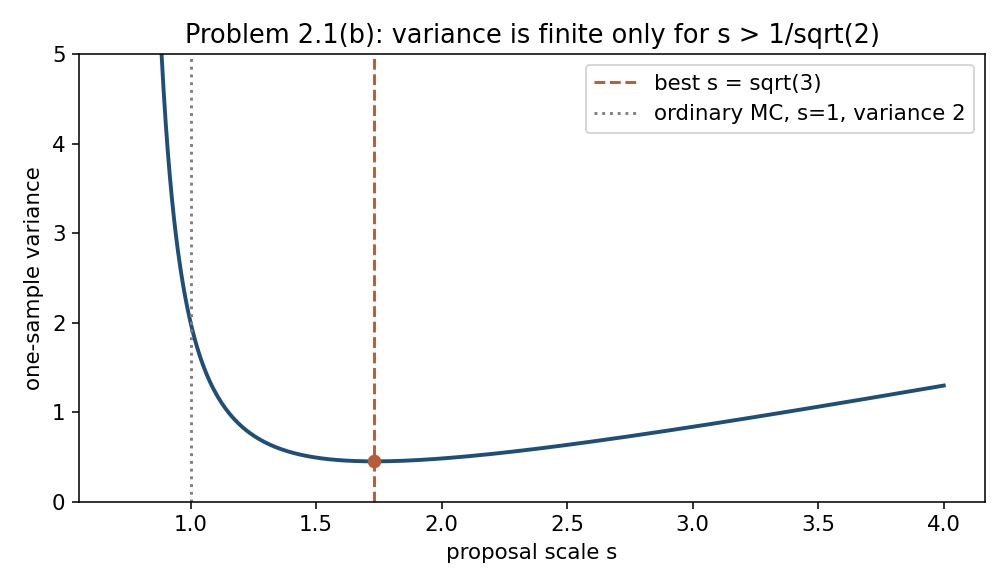
\includegraphics[width=0.62\textwidth]{HW1_figures/importance_variance.png}
\caption{One-sample importance-sampling variance as a function of the proposal scale. The pole at \(s=1/\sqrt{2}\) is where the second moment stops existing. The minimum is at \(s=\sqrt{3}\).}
\end{figure}

\subsection*{2.2 Perplexity}
\addcontentsline{toc}{subsection}{2.2 Perplexity}

Let \(\ell(x)=-\log p_\theta(x)\), \(\widehat{\mathrm{PPL}}_N=\exp(N^{-1}\sum_n\ell(x_n))\), and \(\mathrm{PPL}=\exp(\E[\ell])\), with \(x_n\sim p_{\mathrm{data}}\). The exponential is convex, so Jensen's inequality gives
\[
\E[\widehat{\mathrm{PPL}}_N]\ge\exp(\E[\ell])=\mathrm{PPL}
\]
for every finite \(N\). Equality holds if and only if \(\ell(x)\) is \(p_{\mathrm{data}}\)-almost surely constant. The estimator is therefore not unbiased, except in that trivial case.

If \(\E|\ell|<\infty\), the weak law gives \(N^{-1}\sum\ell(x_n)\to\E[\ell]\) in probability, and the continuous map \(\exp\) preserves convergence in probability. So \(\widehat{\mathrm{PPL}}_N\to\mathrm{PPL}\) in probability: the estimator is consistent.

\subsection*{2.2(a) The \texorpdfstring{\(1/N\)}{1/N} bias}
\addcontentsline{toc}{subsection}{2.2(a) The 1/N bias}

Assume \(\E|\ell|^3<\infty\). Write \(\delta_N=\bar\ell_N-\E[\ell]\). Then \(\E\delta_N=0\), \(\E\delta_N^2=\Var(\ell)/N\), and \(\E\delta_N^3=O(1/N^2)\). The exponential series gives
\[
\E[e^{\delta_N}]=1+\frac{\Var(\ell)}{2N}+o(N^{-1}).
\]
Hence \(\E[\widehat{\mathrm{PPL}}_N]=\mathrm{PPL}\,(1+c/N+o(1/N))\) with \(c=\Var(\ell)/2\).

\subsection*{2.2(b) Gaussian closed form}
\addcontentsline{toc}{subsection}{2.2(b) Gaussian closed form}

Let \(p_{\mathrm{data}}=\N(0,s^2)\), \(p_\theta=\N(0,\sigma^2)\), and \(r=s^2/\sigma^2\). Then
\[
\ell(x)=\tfrac12\log(2\pi\sigma^2)+\frac{x^2}{2\sigma^2},\qquad
\mathrm{PPL}=\sqrt{2\pi\sigma^2}\,e^{r/2}.
\]
With \(\sum_n x_n^2=s^2\chi^2_N\),
\[
\widehat{\mathrm{PPL}}_N=\sqrt{2\pi\sigma^2}\,\exp\big(\tfrac{r}{2N}\chi^2_N\big).
\]
The chi-squared mgf at \(\lambda=r/(2N)\) exists if and only if \(N>r\), and then
\[
\E[\widehat{\mathrm{PPL}}_N]
=\sqrt{2\pi\sigma^2}\,(1-r/N)^{-N/2}.
\]
Expanding \(\log(1-r/N)\) shows the coefficient of \(1/N\) is \(r^2/4\). Independently, \(\Var(\ell)=r^2/2\), so \(\Var(\ell)/2=r^2/4\). This matches 2.2(a). If \(r>1\) the model is narrower than the data, and \(\E[\widehat{\mathrm{PPL}}_N]=\infty\) for every \(N\le r\): the exponential moment does not exist until the sample is larger than \(r\).

\subsection*{2.3 Jensen--Shannon}
\addcontentsline{toc}{subsection}{2.3 Jensen--Shannon}

With \(m=(p+q)/2\),
\[
\JS(p\|q)
=H(m)-\tfrac12 H(p)-\tfrac12 H(q).
\]
Let \(Z\sim\Ber(1/2)\) and \(X\mid Z=0\sim p\), \(X\mid Z=1\sim q\). Then \(I(Z;X)=\JS(p\|q)\). In nats, \(0\le I(Z;X)\le H(Z)=\log 2\). The lower bound holds exactly when \(p=q\). The upper bound holds exactly when \(p\) and \(q\) are mutually singular.

\subsection*{2.3(a) A pointwise bound, and an infinite KL}
\addcontentsline{toc}{subsection}{2.3(a) A pointwise bound, and an infinite KL}

Since \(m\ge p/2\) on \(\{p>0\}\), one has \(\log(p/m)\le\log 2\), so \(\KL(p\|m)\le\log 2\). The same bound for \(q\), averaged, recovers \(\JS\le\log 2\).

JS stays finite when KL does not. Take \(p=\delta_0\) and \(q=\delta_1\) on \(\{0,1\}\). Then \(\KL(p\|q)=\infty\) because \(q(0)=0\) while \(p(0)=1\), but the supports are disjoint, so \(\JS(p\|q)=\log 2\), the maximum.

The bound \(0\le\JS\le 1\) is sharp when \(\log\) is base \(2\). In nats the supremum is \(\ln 2\), and the upper bound \(1\) is valid but not sharp.

\subsection*{2.4 Bernoulli KL at the boundary}
\addcontentsline{toc}{subsection}{2.4 Bernoulli KL at the boundary}

For \(a\in(0,1)\) and \(c\to 0^+\),
\[
\KL(\Ber(a)\|\Ber(c))
=a\log\frac{a}{c}+(1-a)\log\frac{1-a}{1-c}
=a\log\frac{1}{c}+a\log a+(1-a)\log(1-a)+o(1).
\]
The leading term is \(a\log(1/c)\), which diverges. The constant term after it is \(-H(\Ber(a))\), up to the vanishing \(\log(1-c)\). In the other direction,
\[
\KL(\Ber(c)\|\Ber(a))
=c\log\frac{c}{a}+(1-c)\log\frac{1-c}{1-a}
\to -\log(1-a),
\]
which is finite. KL is not symmetric: one direction explodes and the other converges.

\subsection*{2.4(a) No triangle inequality}
\addcontentsline{toc}{subsection}{2.4(a) No triangle inequality}

KL does not satisfy the triangle inequality. For \(1>a>b>0\) and \(c\to 0^+\),
\[
\KL(\Ber(a)\|\Ber(c))\to\infty,
\]
while \(\KL(\Ber(a)\|\Ber(b))\) stays fixed and \(\KL(\Ber(b)\|\Ber(c))\) grows like \(b\log(1/c)\). Since \(a>b\), the left side is eventually larger than the sum of the two right-hand sides. A numerical triple: \(a=1/2\), \(b=1/5\), \(c=1/100\). Then
\[
\KL(a\|c)\approx 1.6145
> 
\KL(a\|b)+\KL(b\|c)\approx 0.6518.
\]

\begin{figure}[ht]
\centering
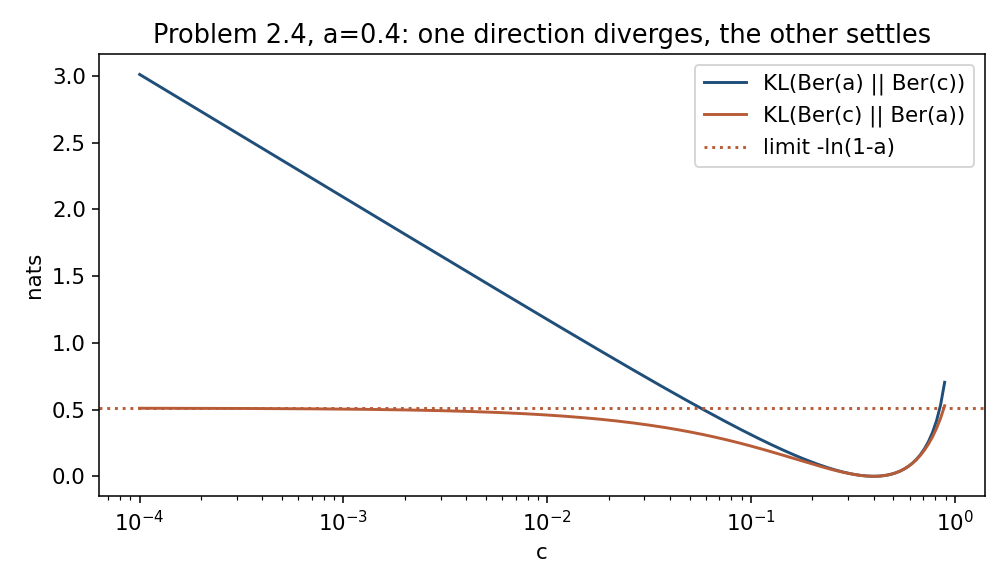
\includegraphics[width=0.7\textwidth]{HW1_figures/kl_asymmetry.png}
\caption{The two directions of Bernoulli KL as the second parameter approaches the boundary. One diverges and one converges, so the triangle inequality cannot hold.}
\end{figure}

\newpage
%----------------------------------------------------------------------
\section{Problem 3, step by step}
%----------------------------------------------------------------------

Context length at position \(i\) is \(\ell_i=\min(m,i-1)\). A conditional table on \(K\) symbols has \(K-1\) free entries per context.

\subsection*{3.1 Two families of Markov models}
\addcontentsline{toc}{subsection}{3.1 Two families of Markov models}

Summing \((K-1)K^{\ell_i}\) over the \(n\) positions,
\[
N_m^{\mathrm{nh}}=(K^m-1)+(n-m)(K-1)K^m.
\]
Checks: \(m=0\) gives \(n(K-1)\), a separate marginal at each position. The case \(m=n-1\) gives \(K^n-1\), an arbitrary positive pmf.

The homogeneous subfamily has an arbitrary prefix of length \(m\), costing \(K^m-1\), and one shared kernel, costing \(K^m(K-1)\):
\[
N_m^{\mathrm{h}}=K^{m+1}-1.
\]
The difference is \((n-m-1)(K-1)K^m\). When \(n=m+1\) the difference is \(0\): only one index uses the kernel, so the two families are the same set, both equal to the full simplex.

\subsection*{3.1(a) Mixture transition model}
\addcontentsline{toc}{subsection}{3.1(a) Mixture transition model}

The model sets \(\Pr(x_i=1\mid x_{i-1}=a,\,x_{i-2}=b)=c_{ab}=\lambda t_1(a)+(1-\lambda)t_2(b)\), with five nominal parameters, while a free table has four entries. The cross difference vanishes:
\[
c_{00}-c_{01}-c_{10}+c_{11}=0.
\]
Conversely, every \(c\in[0,1]^4\) on this hyperplane is attained. Additivity gives \(c_{ab}=A_a+B_b\). Taking \(B_b=\min_a c_{ab}\) and \(A_a=c_{ab}-B_b\) produces nonnegative summands, and rescaling them into \(\lambda\in[0,1]\) and two maps \(t_1,t_2\) hits \(c\). The image is a full-dimensional subset of a \(3\)-dimensional affine subspace of \(\R^4\), cut by the cube. Its dimension is \(3\).

Five parameters mapping onto a \(3\)-dimensional set overcount. A generic fiber has dimension \(5-3=2\). The model cannot represent a conditional with a nonzero interaction, for example \(c=(1,0,0,1)\).

\subsection*{3.2 Closest autoregressive tables}
\addcontentsline{toc}{subsection}{3.2 Closest autoregressive tables}

Let \(q(x)=\prod_i q_i(x_i\mid c_i)\) and let \(q^\star(x)=\prod_i p(x_i\mid c_i)\) use the conditionals of \(p\) itself. The chain rule gives
\[
\KL(p\|q)
=\KL(p\|q^\star)
+\sum_{i=1}^n\E\big[\KL(p(\cdot\mid c_i)\,\|\,q_i(\cdot\mid c_i))\big].
\]
Each inner KL is nonnegative. So \(\KL(p\|q)\ge\KL(p\|q^\star)\), with equality if and only if every table of \(q\) matches the corresponding conditional of \(p\). Since \(p>0\), every context occurs, and the closest member of the inhomogeneous family is unique: it is \(q^\star\).

\subsection*{3.2(a) The gap is a sum of conditional mutual informations}
\addcontentsline{toc}{subsection}{3.2(a) The gap is a sum of conditional mutual informations}

For \(i\le m+1\) the window \(c_i\) is the entire past, so those terms cancel between \(p\) and \(q^\star\). For \(i\ge m+2\),
\[
\KL(p\|q^\star)
=\sum_{i=m+2}^{n}I\big(X_i;\,X_{1:i-m-1}\mid X_{i-m:i-1}\big).
\]
The gap is zero if and only if \(p\) itself factors through windows of length \(m\). For \(m=0\),
\[
\KL(p\|q^\star)=\sum_{i=2}^n I(X_i;X_{1:i-1}),
\]
the total correlation of \(p\).

\subsection*{3.2(b) Maximum likelihood tables}
\addcontentsline{toc}{subsection}{3.2(b) Maximum likelihood tables}

The average log-likelihood of \(N\) i.i.d.\ sequences separates across positions and contexts:
\[
\sum_i\sum_{c,k}\hat p_i(c,k)\log q_i(k\mid c).
\]
For each \((i,c)\) with a positive count, the Lagrangian under \(\sum_k q_k=1\) has solution
\[
\hat q_i(k\mid c)=\frac{N_i(c,k)}{N_i(c)}.
\]
These are the conditionals of the empirical distribution. Maximizing the likelihood is the same as minimizing \(\KL(\hat p\|q)\), whose unique minimizer on the observed contexts is the \(q^\star\) of 3.2 built from \(\hat p\). Unseen contexts are unidentified.

\subsection*{3.2(c) Best homogeneous model}
\addcontentsline{toc}{subsection}{3.2(c) Best homogeneous model}

The prefix log-likelihood is maximized by the true marginal \(\pi^\star=p_{1:m}\). The shared kernel maximizes \(\sum_{i>m}\sum_{c,k}p_i(c,k)\log T(k\mid c)\), so
\[
T^\star(k\mid c)
=\sum_{i=m+1}^n w_i(c)\,p_i(k\mid c),
\qquad
w_i(c)=\frac{p_i(c)}{\sum_{j>m}p_j(c)}.
\]
It is the average of the position-wise conditionals, weighted by how often the context occurs. The extra KL above 3.2(a) is
\[
\sum_{i=m+1}^n\sum_c p_i(c)\,\KL\big(p_i(\cdot\mid c)\,\|\,T^\star(\cdot\mid c)\big).
\]
It vanishes if and only if \(p_i(\cdot\mid c)\) does not depend on \(i\), which is homogeneity of order \(m\).

\subsection*{3.3 The graph in Figure 1}
\addcontentsline{toc}{subsection}{3.3 The graph in Figure 1}

Parents, read from the figure: \(A\) and \(B\) are roots, \(\pa(C)=\pa(D)=\{A\}\), \(\pa(E)=\{B\}\), \(\pa(F)=\{C,D\}\), \(\pa(G)=\{B,E\}\). Therefore
\begin{align*}
p(x)&=p(x_A)\,p(x_B)\,p(x_C\mid x_A)\,p(x_D\mid x_A)\\
&\quad\cdot p(x_E\mid x_B)\,p(x_F\mid x_C,x_D)\,p(x_G\mid x_B,x_E).
\end{align*}
Binary tables contribute \(2^{|\pa(v)|}\) free parameters:
\[
1+1+2+2+2+4+4=16.
\]

Normalization. Induct along a topological order. Each conditional sums to \(1\) for every parent configuration, and the parents appear earlier in the order, so summing out the next variable leaves a pmf. After all seven variables the product sums to \(1\). Acyclicity is what supplies the order.

\subsection*{3.3(a) Valid orderings}
\addcontentsline{toc}{subsection}{3.3(a) Valid orderings}

On \(\{B,E,G\}\) the only topological order is \(B,E,G\). On \(\{A,C,D,F\}\), node \(A\) is first, \(F\) is last, and \(\{C,D\}\) is free: \(2\) orders. Interleaving the two blocks,
\[
\binom{7}{3}\cdot 1\cdot 2=70.
\]
Out of \(7!=5040\) permutations, the proportion is \(70/5040=1/72\).

\subsection*{3.3(b) The same count from a rooted forest}
\addcontentsline{toc}{subsection}{3.3(b) The same count from a rooted forest}

For a rooted tree in which every node has at most one parent and edges point away from the root, the number of orders in which every node precedes its descendants is \(n!/\prod_v h_v\), where \(h_v\) is the subtree size at \(v\). A forest is an interleaving of its trees, and the same formula holds for the whole vertex set.

Delete \(C\to F\) and \(E\to G\). The forest has subtree sizes \(h_B=3\), \(h_E=h_G=1\), \(h_A=4\), \(h_D=2\), \(h_C=h_F=1\), so
\[
\prod_v h_v=24,\qquad 7!/24=210.
\]
Restoring an edge keeps the forest orders that also put the new parent before the child.
\begin{itemize}
\item Restoring \(E\to G\): \(E\) and \(G\) are symmetric leaves, so exactly half of the orders survive. Count \(105\).
\item Restoring \(C\to F\): among the orders with \(D\) before \(F\), two of the three equally likely placements of \(C\) put \(C\) before \(F\). Fraction \(2/3\), count \(140\).
\item Restoring both: the two constraints use disjoint vertices, so the fractions multiply. Fraction \(1/3\), count \(70\).
\end{itemize}
The both-edges count \(70\) is exactly the direct count of 3.3(a). That is the comparison the problem asks for.

\subsection*{3.3(c) A directed cycle does not normalize}
\addcontentsline{toc}{subsection}{3.3(c) A directed cycle does not normalize}

On two binary variables, the product of the two cyclic conditionals has atoms
\begin{align*}
q(0,0)&=(1-\theta_0)(1-\varphi_0),&
q(1,0)&=\theta_0(1-\varphi_1),\\
q(0,1)&=(1-\theta_1)\varphi_0,&
q(1,1)&=\theta_1\varphi_1.
\end{align*}
Their sum is
\[
Z=1+(\theta_0-\theta_1)(\varphi_0-\varphi_1).
\]
At \((\theta_0,\theta_1,\varphi_0,\varphi_1)=(0.2,0.8,0.3,0.9)\) this equals \(1.36\). So \(Z=1\) for every parameter if and only if \(\theta_0=\theta_1\) or \(\varphi_0=\varphi_1\), i.e.\ at least one conditional ignores its parent.

Maximum likelihood needs \(\sum_x\log(q_\theta(x)/Z(\theta))\). Dropping \(\log Z(\theta)\) is not the log-likelihood as soon as \(Z\) depends on \(\theta\). The score misses \(-\nabla\log Z\), and the parameters stay coupled through the normalizer. A DAG factorization would have avoided that coupling.

\newpage
%----------------------------------------------------------------------
\section{Problem 4, step by step}
%----------------------------------------------------------------------

\subsection*{4.1 Parameter counts}
\addcontentsline{toc}{subsection}{4.1 Parameter counts}

FVSBN: one bias per coordinate and a weight vector \(w_d\in\R^{d-1}\),
\[
\frac{D(D+1)}{2}.
\]
At \(D=784\) this is \(307720\).

NADE: \(W\) contributes \(D_h(D-1)\), the shared bias \(c\) contributes \(D_h\), each of the \(D-1\) later conditionals contributes a vector \(v_d\) and a bias, and \(b_1\) is one more bias,
\[
D_h(2D-1)+D.
\]
NADE is smaller when \(D_h<D(D-1)/(2(2D-1))\). For \(D=784\) the threshold is \(306936/1567\approx 195.875\), so the largest such integer is \(D_h=195\).

\subsection*{4.1(a) Scalar multiplications}
\addcontentsline{toc}{subsection}{4.1(a) Scalar multiplications}

Count products inside the affine maps, not evaluations of \(\sigma\), \(\log\), or \(\phi\).
\begin{itemize}
\item FVSBN: \(\sum_{d=2}^D(d-1)=D(D-1)/2\). At \(D=784\): \(306936\).
\item NADE, recomputing each \(a_d\): \(D_h(D-1)(D+2)/2\). At \(D=784\), \(D_h=500\): \(153859500\).
\item NADE, with \(a_{d+1}=a_d+W_{:,d}x_d\): \(2(D-1)D_h\). At the same size: \(783000\).
\end{itemize}

\subsection*{4.1(b) Sampling stays sequential}
\addcontentsline{toc}{subsection}{4.1(b) Sampling stays sequential}

To sample \(x_d\) one needs \(a_d\), which depends on \(x_1,\ldots,x_{d-1}\). Those bits are not known until the previous draws have been made. The recursion removes repeated arithmetic. It does not remove the chain. For a fixed observed \(x\), every bit is already known, so the \(D\) conditionals may be evaluated independently.

\subsection*{4.2 NADE gradients}
\addcontentsline{toc}{subsection}{4.2 NADE gradients}

The Bernoulli negative log-likelihood in the logit has derivative \(\delta_d=\sigma(z_d)-x_d\). With \(z_1=b_1\) and \(z_d=v_d^\top h_d+b_d\),
\begin{align*}
\frac{\partial L}{\partial b_d}&=\delta_d, &
\frac{\partial L}{\partial v_d}&=\delta_d h_d\ (d\ge 2),\\
\frac{\partial L}{\partial h_d}&=\delta_d v_d, &
\frac{\partial L}{\partial a_d}&=\phi'(a_d)\odot(\delta_d v_d).
\end{align*}
The bias \(b_d\) and the vector \(v_d\) touch only conditional \(d\). The shared parameters touch every later conditional:
\[
\frac{\partial L}{\partial c}=\sum_{d=2}^D\frac{\partial L}{\partial a_d},\qquad
\frac{\partial L}{\partial W_{:,k}}=x_k\sum_{d=k+1}^D\frac{\partial L}{\partial a_d}.
\]

\subsection*{4.2(a) One backward pass, MAP, tanh symmetry}
\addcontentsline{toc}{subsection}{4.2(a) One backward pass, MAP, tanh symmetry}

Write \(g_d=\partial L/\partial a_d\). After one forward pass, set \(S_{D-1}=g_D\) and \(S_k=g_{k+1}+S_{k+1}\) while \(k\) runs downward. Then \(\partial L/\partial W_{:,k}=x_k S_k\). The accumulation costs the same order as one forward pass.

With \(N\) observations and prior \(\theta\sim\N(0,\tau^2 I)\), the negative log posterior, up to a constant, is
\[
J(\theta)=\sum_{n=1}^N L(x^{(n)};\theta)+\frac{1}{2\tau^2}\lVert\theta\rVert^2.
\]
The extra gradient \(\theta/\tau^2\) is weight decay with coefficient \(1/\tau^2\).

Symmetries for \(\phi=\tanh\), which is odd. For each hidden unit \(j\) and each sign \(\varepsilon_j\in\{\pm 1\}\), flip the sign of \(c_j\), of row \(j\) of \(W\), and of coordinate \(j\) of every \(v_d\). Then \(a_{d,j}\) and \(h_{d,j}\) both change sign, and \(v_d^\top h_d\) is unchanged. Any common permutation of the hidden coordinates does the same. Together these form a group of order \(D_h!\,2^{D_h}\). For a generic \(\theta\) the images are distinct, so a generic fiber contains at least that many parameter vectors. This is the size of the generic fiber, not a lower bound that holds for every \(\theta\): some special \(\theta\) have a smaller orbit.

\subsection*{4.3 What an FVSBN can represent}
\addcontentsline{toc}{subsection}{4.3 What an FVSBN can represent}

The logits \(\ell_d(x_{<d})=\log p(x_d=1\mid x_{<d})/p(x_d=0\mid x_{<d})\) may be arbitrary real functions for a general positive pmf. An FVSBN forces each logit to be affine. So \(\mathcal{F}_D\) is exactly the set of positive pmfs whose autoregressive logits, in the fixed order, are affine.

The map from parameters to pmfs is injective: an affine function on the cube determines its coefficients by finite differences, \(b=\ell(0)\) and \(w_i=\ell(e_i)-\ell(0)\). The parameter count is \(D(D+1)/2\), so \(\dim\mathcal{F}_D=D(D+1)/2\). The full simplex has dimension \(2^D-1\). Equality holds for \(D=1\) and \(D=2\) only.

\subsection*{4.3(a) Parity is not an FVSBN}
\addcontentsline{toc}{subsection}{4.3(a) Parity is not an FVSBN}

Let \(p(x)=\theta/4\) when \(x_1\oplus x_2\oplus x_3=1\) and \((1-\theta)/4\) otherwise, with \(\theta=0.1\). Four odd strings and four even strings, and the masses sum to \(1\). By symmetry it is enough to rule out one order.

The marginal of \((x_1,x_2)\) is uniform. The conditional probability of \(x_3=1\) equals \(\theta\) when \(x_1\oplus x_2=0\) and equals \(1-\theta\) otherwise. With \(L=\log(\theta/(1-\theta))=\log(1/9)\),
\[
\ell(0,0)=\ell(1,1)=L,\qquad\ell(1,0)=\ell(0,1)=-L.
\]
The second-order interaction is
\[
\ell(1,1)-\ell(1,0)-\ell(0,1)+\ell(0,0)=4L=-4\log 9\ne 0.
\]
An affine logit would have given \(0\). No FVSBN represents \(p\), in any order.

\subsection*{4.3(b) Parity with a ReLU NADE of width \texorpdfstring{\(D-1\)}{D-1}}
\addcontentsline{toc}{subsection}{4.3(b) Parity with a ReLU NADE of width D-1}

Yes. Let \(L=\log(\theta/(1-\theta))\) and \(D_h=D-1\). Set \(b_1=0\), and \(v_d=0\), \(b_d=0\) for \(2\le d\le D-1\). Then the first \(D-1\) bits are i.i.d.\ fair, regardless of \(W\) and \(c\).

For the last conditional, use one hidden unit per threshold: \(c_j=1-j\) and \(W=\mathbf{1}\). Then \(a_{D,j}=s-(j-1)\) with \(s=\sum_{k<D}x_k\), and \(h_j=\ReLU(s-(j-1))\). On integers these ReLUs reproduce the indicators \(\mathbf{1}_{s\ge k}\) by differences, and any function of the integer \(s\) is linear in \(h\). Taking the function \(L(-1)^s\) gives
\[
b_D=L,\qquad v_{D,1}=-2L,\qquad v_{D,j}=4L(-1)^j\ (j\ge 2).
\]
Then \(z_D=L\) on even popcount and \(z_D=-L\) on odd popcount, so the conditional probability that the total parity is odd equals \(\theta\).

\subsection*{4.4 Masks for Figure 2}
\addcontentsline{toc}{subsection}{4.4 Masks for Figure 2}

Columns of \(M^W\) are \((x_1,x_2,x_3,x_4)\) with degrees \((2,4,1,3)\). Rows are \(h_1,\ldots,h_6\) with degrees \((1,3,3,1,3,1)\):
\[
M^W=\begin{pmatrix}
0&0&1&0\\
1&0&1&1\\
1&0&1&1\\
0&0&1&0\\
1&0&1&1\\
0&0&1&0
\end{pmatrix},
\qquad
\#\{1\}=12.
\]
Rows of \(M^V\) are \(\lambda_1,\ldots,\lambda_4\):
\[
M^V=\begin{pmatrix}
1&0&0&1&0&1\\
1&1&1&1&1&1\\
0&0&0&0&0&0\\
1&0&0&1&0&1
\end{pmatrix},
\qquad
\#\{1\}=12.
\]
Hidden unit \(k\) sees inputs of degree at most \(m^1(k)\), and output \(d\) sees hidden units of degree strictly less than \(m^0(d)\). So \(\lambda_d\) depends only on inputs of degree \(<m^0(d)\). In the order \(x_3,x_1,x_4,x_2\):
\begin{center}
\begin{tabular}{@{}lll@{}}
\toprule
conditional & earlier variables the order allows & variables with a path \\
\midrule
\(\lambda_3\) & none & none \\
\(\lambda_1\) & \(x_3\) & \(x_3\) \\
\(\lambda_4\) & \(x_3,x_1\) & \(x_3\) only \\
\(\lambda_2\) & \(x_3,x_1,x_4\) & \(x_3,x_1,x_4\) \\
\bottomrule
\end{tabular}
\end{center}
The missing dependence is \(x_1\to\lambda_4\). A hidden unit that sees \(x_1\) needs degree at least \(2\), but \(\lambda_4\) accepts only degrees strictly less than \(3\). Figure~2 has no hidden unit of degree \(2\).

The network is not as expressive as a general autoregressive model for this order. For general \(D\) and one hidden layer, the consecutive dependence \(r\to r+1\) forces a hidden unit of degree exactly \(r\). These \(D-1\) requirements are disjoint, so \(H\ge D-1\). One unit of each degree \(1,\ldots,D-1\) meets every interval, so \(H=D-1\) is also sufficient for connectivity. A single hidden layer of that width still cannot match an arbitrary conditional table. What it does not lose is any dependence the ordering itself permits.

\subsection*{4.4(a) Any depth, and the non-strict output rule}
\addcontentsline{toc}{subsection}{4.4(a) Any depth, and the non-strict output rule}

Use the same inequality between successive hidden layers. By induction, a unit of degree \(m\) depends only on inputs of degree at most \(m\). The output \(\lambda_d\) reads only units of degree \(<m^0(d)\), hence only inputs of degree \(<m^0(d)\). It does not depend on \(x_d\) or on any later variable. Each factor is a conditional probability given the earlier variables in the degree order, and summing from the last variable back to the first shows that \(p\) is a pmf.

If the output rule is weakened to \(\mathbf{1}\{m^0(d)\ge m^1(k)\}\), a unit of degree \(m^0(d)\) may connect to \(\lambda_d\) and may depend on \(x_d\). Then \(\lambda_d\) depends on \(x_d\), and summing the Bernoulli factor in \(x_d\) need not give \(1\). In Figure~2 this happens for \(\lambda_3\), through \(h_1,h_4,h_6\), and for \(\lambda_4\), through \(h_2,h_3,h_5\).

\subsection*{4.4(b) Random hidden degrees}
\addcontentsline{toc}{subsection}{4.4(b) Random hidden degrees}

Degrees are i.i.d.\ uniform on \(\{1,\ldots,D-1\}\). For an input of degree \(r\), \(\Pr(m^1\ge r)=(D-r)/(D-1)\). Summing over \(r\) gives \(D/2\). With \(H\) independent rows,
\[
\E[\#\{M^W=1\}]=\frac{HD}{2},
\]
and the same count holds for \(M^V\).

An allowed dependence \(r\to j\), with \(j>r\), is connected when at least one hidden degree falls in an interval of \(j-r\) integers:
\[
\Pr(\text{connected})=1-\Big(1-\frac{j-r}{D-1}\Big)^H.
\]
All allowed dependences are connected simultaneously if and only if every degree in \(\{1,\ldots,D-1\}\) appears at least once. This is the coupon collector on \(D-1\) coupons. The expected number of hidden units until every degree has appeared is
\[
(D-1)\,H_{D-1},
\]
where \(H_{D-1}\) is the harmonic number. At \(D=784\),
\[
783\,H_{783}\approx 5669.69.
\]

\newpage
%----------------------------------------------------------------------
\section{Problem 5, step by step}
%----------------------------------------------------------------------

Recall \(\ell(x;\mu,s)=\tfrac12\log(2\pi)+s/2+(x-\mu)^2 e^{-s}/2\), and
\[
\delta^\mu=-(x-\mu)e^{-s},\qquad
\delta^s=\tfrac12-\tfrac12(x-\mu)^2 e^{-s}.
\]

\subsection*{5.1 Gradients}
\addcontentsline{toc}{subsection}{5.1 Gradients}

One conditional contributes \(\delta^\mu\) to its mean and \(\delta^s\) to its log-variance. The chain rule through \(\mu_d=v_d^\top h_d+b_d\) and \(s_d=u_d^\top h_d+e_d\) gives
\begin{align*}
\frac{\partial L}{\partial b_d}&=\delta^\mu_d, &
\frac{\partial L}{\partial v_d}&=\delta^\mu_d\,h_d, &
\frac{\partial L}{\partial e_d}&=\delta^s_d, &
\frac{\partial L}{\partial u_d}&=\delta^s_d\,h_d,\\
\frac{\partial L}{\partial h_d}&=\delta^\mu_d\,v_d+\delta^s_d\,u_d, &
\frac{\partial L}{\partial a_d}&=\phi'(a_d)\odot\frac{\partial L}{\partial h_d}.
\end{align*}
The shared parameters accumulate exactly as in NADE, with \(\partial L/\partial a_d\) in place of the Bernoulli backpropagated vector:
\[
\frac{\partial L}{\partial c}=\sum_{d\ge 2}\frac{\partial L}{\partial a_d},\qquad
\frac{\partial L}{\partial W_{:,k}}=x_k\sum_{d>k}\frac{\partial L}{\partial a_d}.
\]
For \(d=1\) there is no hidden state: \(\partial L/\partial b_1=\delta^\mu_1\) and \(\partial L/\partial e_1=\delta^s_1\).

\subsection*{5.1(a) A constant Gaussian fit}
\addcontentsline{toc}{subsection}{5.1(a) A constant Gaussian fit}

For i.i.d.\ scalars from \(\N(\mu_0,\sigma_0^2)\), the average negative log-likelihood of a constant \((\mu,s)\) is minimized at the empirical mean and the empirical second moment. The critical point \(\hat\mu=\bar x\), \(e^{\hat s}=N^{-1}\sum_n(x_n-\bar x)^2\) is the unique global minimum, because the loss is the Gaussian KL up to a constant and that KL is zero only at the true moments of the empirical measure. The fitted variance is biased:
\[
\E[e^{\hat s}]=\sigma_0^2\frac{N-1}{N}.
\]

\subsection*{5.2 Hessian}
\addcontentsline{toc}{subsection}{5.2 Hessian}

Differentiating \(\delta^\mu\) and \(\delta^s\) once more produces
\[
\nabla^2\ell
=\begin{pmatrix}
e^{-s} & (x-\mu)e^{-s}\\
(x-\mu)e^{-s} & \tfrac12(x-\mu)^2 e^{-s}
\end{pmatrix}.
\]
The determinant equals \(-\tfrac12(x-\mu)^2 e^{-2s}\le 0\), and it is strictly negative when \(x\ne\mu\). The Hessian is then indefinite. The loss is not jointly convex in \((\mu,s)\), and not jointly concave either.

\subsection*{5.2(a) Natural parameters}
\addcontentsline{toc}{subsection}{5.2(a) Natural parameters}

Set \(\eta_1=\mu e^{-s}\) and \(\eta_2=-\tfrac12 e^{-s}\), so \(\eta_2<0\). Completing the square,
\[
\N(x\mid\mu,e^s)
=\frac{1}{\sqrt{2\pi}}\exp(\eta_1 x+\eta_2 x^2-A(\eta)),
\]
\[
A(\eta)=-\tfrac12\log(-2\eta_2)-\frac{\eta_1^2}{4\eta_2}.
\]
Hence \(\ell=\tfrac12\log(2\pi)-\eta_1 x-\eta_2 x^2+A(\eta)\). The terms in \(x\) are linear in \(\eta\). The Hessian of \(A\) is positive definite on \(\{\eta_2<0\}\):
\[
\partial_{\eta_1\eta_1}A=\frac{1}{-2\eta_2}>0,\qquad
\det\nabla^2 A=-\frac{1}{4\eta_2^3}>0.
\]
So \(A\), and therefore \(\ell\), is strictly convex in \(\eta\).

\subsection*{5.2(b) Separate convexity, and the network parameters}
\addcontentsline{toc}{subsection}{5.2(b) Separate convexity, and the network parameters}

For fixed \(s\), \(\partial^2\ell/\partial\mu^2=e^{-s}>0\): strictly convex in \(\mu\). For fixed \(\mu\), \(\partial^2\ell/\partial s^2=\tfrac12(x-\mu)^2 e^{-s}\ge 0\): convex in \(s\).

If \((u_d,e_d,h_d)\) are held fixed, \(\mu_d\) is affine in \((v_d,b_d)\). A convex function of an affine map is convex, so the NLL is convex in \((v_d,b_d)\). Likewise, with everything else fixed, the NLL is convex in \((u_d,e_d)\).

It is not jointly convex in \((v_d,u_d)\). If \(h_d\ne 0\), the map \((v_d,u_d)\mapsto(\mu_d,s_d)\) is linear and surjective onto \(\R^2\). Joint convexity would imply joint convexity in \((\mu,s)\), which 5.2 forbids. Explicitly, \(h_d=1\), \(b_d=e_d=0\), \(x=0\), \(\mu=1\), \(s=0\): the Hessian in \((\mu,s)\) has determinant \(-1/2<0\).

\subsection*{5.3 One dimension}
\addcontentsline{toc}{subsection}{5.3 One dimension}

One training point. Set \(\mu=x\) and let \(s\to-\infty\). Then \(\ell=s/2+\tfrac12\log(2\pi)\to-\infty\). The NLL is not bounded below.

\(N\ge 2\) distinct points. Let \(S=\sum_n(x_n-\bar x)^2>0\). For every \((\mu,s)\),
\[
\sum_{n=1}^N\ell(x_n;\mu,s)\ge\frac N2\log\Big(2\pi e\frac{S}{N}\Big),
\]
with equality at \(\mu=\bar x\) and \(e^s=S/N\). This is the greatest lower bound, and it is attained. The average NLL is bounded below by \(\tfrac12\log(2\pi e\,S/N)\).

\subsection*{5.3(a) A two-dimensional conditional has no floor}
\addcontentsline{toc}{subsection}{5.3(a) A two-dimensional conditional has no floor}

No. The first coordinates are distinct, and the hidden layer is wide enough to interpolate arbitrary values of \((\mu_2,s_2)\) at those finitely many inputs. Set \(\mu_2(x_{n1})=x_{n2}\) and send \(s_2(x_{n1})\to-\infty\) at each training input. Every conditional term \((x_{n2}-\mu_2)^2 e^{-s_2}\) vanishes while \(s_2/2\to-\infty\), so the training NLL tends to \(-\infty\).

A discrete model cannot do this. For any pmf \(q\),
\[
-\E_{p_{\mathrm{data}}}\log q=H(p_{\mathrm{data}})+\KL(p_{\mathrm{data}}\|q)\ge H(p_{\mathrm{data}}).
\]
The average NLL cannot undercut the entropy of the data distribution. Continuous training data are a sum of atoms. A density value at a point can be arbitrarily large, and there is no entropy floor under the empirical measure.

\subsection*{5.3(b) A variance floor restores a bound}
\addcontentsline{toc}{subsection}{5.3(b) A variance floor restores a bound}

The phrase ``change (b)'' in the PDF refers to the unboundedness just proved. With \(s_d\ge s_{\min}\) for every conditional, the squared residual is nonnegative and \(s/2\) is increasing, so
\[
\ell(x_d;\mu_d,s_d)\ge\tfrac12\big(\log(2\pi)+s_{\min}\big).
\]
Summing over the \(D\) coordinates,
\[
-\log p_\theta(x)\ge\frac D2\big(\log(2\pi)+s_{\min}\big)
\]
for every \(x\) and every parameter obeying the floor. The training NLL is bounded below by \(N\) times this constant. The floor is what creates the bound: without it, \(s_2\to-\infty\) was available at the training inputs.

\subsection*{5.4(a) Mixture responsibilities}
\addcontentsline{toc}{subsection}{5.4(a) Mixture responsibilities}

Let \(\varphi_c=\N(x\mid\mu_c,e^{s_c})\), \(Z=\sum_j\pi_j\varphi_j\), \(L=-\log Z\), and \(\gamma_c=\pi_c\varphi_c/Z\), with \(\pi=\softmax(\ell_1,\ldots,\ell_C)\). The softmax Jacobian gives
\[
\frac{\partial L}{\partial\ell_c}=\pi_c-\gamma_c.
\]
These derivatives sum to \(0\): adding a constant to every logit does not change \(\pi\). Differentiating through one component,
\[
\frac{\partial L}{\partial\mu_c}=\gamma_c\,\delta^\mu_c,\qquad
\frac{\partial L}{\partial s_c}=\gamma_c\,\delta^s_c.
\]
Compared with 5.1, each Gaussian gradient is multiplied by the responsibility of that component. Through the heads,
\[
\frac{\partial L}{\partial h}
=\sum_c\Big((\pi_c-\gamma_c)a_c+\gamma_c\delta^\mu_c\,v_c+\gamma_c\delta^s_c\,u_c\Big).
\]
With a single component, \(\gamma=1\) and this reduces to the gradient of 5.1.

\subsection*{5.4(b) The mixture likelihood is unbounded}
\addcontentsline{toc}{subsection}{5.4(b) The mixture likelihood is unbounded}

For \(C\ge 2\) and \(N\ge 2\) distinct points there is no upper bound. Put \(\mu_1=x_1\), send \(s_1\to-\infty\), and keep \(\pi_1=\pi_2=1/2\) with \(s_2\) fixed. The density at \(x_1\) tends to infinity. At every other training point the collapsed component vanishes, but the second component stays at a positive density. The product of the \(N\) mixture densities tends to infinity. For \(C=1\) this escape is impossible, by 5.3.

\subsection*{5.4(c) The mixture NLL is not convex}
\addcontentsline{toc}{subsection}{5.4(c) The mixture NLL is not convex}

Take \(C=2\), one observation \(x=0\), \(\pi=(1/2,1/2)\), \(s_1=s_2=0\), and free means. Up to an additive constant the NLL as a function of \((\mu_1,\mu_2)\) satisfies \(L(0,3)=L(3,0)\), while the midpoint \((1.5,1.5)\) has a strictly larger value:
\[
L(0,3)=L(3,0)\approx -0.011,\qquad L(1.5,1.5)\approx 0.432.
\]
A convex function cannot be larger at the midpoint than at the endpoints. Relabeling the two components does not change the mixture, so each distribution coming from distinct component parameters is represented by at least \(2!=2\) parameter vectors, and by \(C!\) after the same argument with \(C\) components.

\newpage
%----------------------------------------------------------------------
\section{Problem 6, step by step}
%----------------------------------------------------------------------

\subsection*{6.1 Bayes classifier for class-conditional Gaussians}
\addcontentsline{toc}{subsection}{6.1 Bayes classifier for class-conditional Gaussians}

With \(p(y=1)=\pi\) and \(x\mid y=c\sim\N(\mu_c,\Sigma_c)\),
\begin{align*}
a(x)&=\log\frac{\pi}{1-\pi}-\tfrac12\log\frac{\det\Sigma_1}{\det\Sigma_0}\\
&\quad+\tfrac12(x-\mu_0)^\top\Sigma_0^{-1}(x-\mu_0)
-\tfrac12(x-\mu_1)^\top\Sigma_1^{-1}(x-\mu_1),
\end{align*}
and \(p(y=1\mid x)=\sigma(a(x))\).

Shared covariance \(\Sigma_0=\Sigma_1=\Sigma\). The pure quadratic terms cancel. With \(\Delta=\mu_1-\mu_0\) and \(\bar\mu=\tfrac12(\mu_0+\mu_1)\),
\[
a(x)=w^\top x+b,\qquad
w=\Sigma^{-1}\Delta,\qquad
b=-w^\top\bar\mu+\log\frac{\pi}{1-\pi}.
\]
The logit is affine.

Unequal covariances. Expanding leaves a quadratic discriminant,
\begin{align*}
a(x)&=x^\top Q x+L^\top x+c,\\
Q&=\tfrac12(\Sigma_0^{-1}-\Sigma_1^{-1}),\qquad
L=\Sigma_1^{-1}\mu_1-\Sigma_0^{-1}\mu_0,
\end{align*}
with \(c\) collecting \(\log(\pi/(1-\pi))\), the log-determinant, and the two quadratic mean terms.

\subsection*{6.1(a) Parameter counts and the fiber}
\addcontentsline{toc}{subsection}{6.1(a) Parameter counts and the fiber}

Shared-covariance generative model: one \(\pi\in(0,1)\), two means in \(\R^D\), and a covariance of dimension \(D(D+1)/2\). Total
\[
1+2D+\frac{D(D+1)}{2}.
\]
Logistic regression has \(D+1\) parameters, the vector \(w\) and the bias \(b\).

Fix \((w,b)\). Choose any \(\Sigma\succ 0\) and any midpoint \(\bar\mu\). Then \(\Delta=\Sigma w\) is forced, the two means are \(\bar\mu\pm\Delta/2\), and
\[
\log\frac{\pi}{1-\pi}=b+w^\top\bar\mu
\]
determines \(\pi\in(0,1)\). The fiber is diffeomorphic to \(\{\Sigma\succ 0\}\times\R^D\) and has dimension
\[
\frac{D(D+1)}{2}+D=\frac{D(D+3)}{2}.
\]
This equals the difference of the two parameter counts, so every logistic parameter is realized by some generative model.

\subsection*{6.2 The classifier on the observed coordinates}
\addcontentsline{toc}{subsection}{6.2 The classifier on the observed coordinates}

Only the coordinates in \(V\) are observed. Under the shared covariance, the marginal is
\[
x_V\mid y=c\sim\N(\mu_{c,V},\Sigma_{VV}).
\]
Part 6.1 in these coordinates gives
\[
p(y=1\mid x_V)=\sigma(w_V^\top x_V+b_V),
\]
\[
w_V=\Sigma_{VV}^{-1}\Delta_V,\qquad
b_V=-\Delta_V^\top\Sigma_{VV}^{-1}\bar\mu_V+\log\frac{\pi}{1-\pi}.
\]
The Schur complement \(S_{V\mid M}=\Sigma_{VV}-\Sigma_{VM}\Sigma_{MM}^{-1}\Sigma_{MV}\) is the conditional covariance of \(x_V\) given \(x_M\). It is not the covariance of this marginal. The Bayes rule for the masked problem inverts \(\Sigma_{VV}\), not \(S_{V\mid M}\).

\subsection*{6.2(a) Mean imputation is a different coefficient}
\addcontentsline{toc}{subsection}{6.2(a) Mean imputation is a different coefficient}

The full-data classifier has \(w=\Sigma^{-1}\Delta\). Substituting \(x_M\leftarrow\bar\mu_M\) cancels the masked block against the bias and leaves
\[
w_V^\top(x_V-\bar\mu_V)+\log\frac{\pi}{1-\pi},
\]
where \(w_V\) here means the \(V\)-block of \(\Sigma^{-1}\Delta\), not the coefficient of 6.2. The block formula for the inverse says \((\Sigma^{-1})_{VV}=S_{V\mid M}^{-1}\), so the coefficient actually applied to \(x_V\) is
\[
S_{V\mid M}^{-1}\Delta_V
-S_{V\mid M}^{-1}\Sigma_{VM}\Sigma_{MM}^{-1}\Delta_M.
\]
The Bayes-optimal coefficient of 6.2 is \(\Sigma_{VV}^{-1}\Delta_V\). They agree for every \(x_V\) if and only if the two coefficient vectors are equal. That happens when the missing block carries no extra information about the class gap, in particular when \(\Sigma_{VM}=0\), and more generally when \(\Delta_M\) equals the regression of \(\Delta_V\) that the cross-covariance would predict. Otherwise, filling the hole with \(\bar\mu_M\) is not the same classifier as throwing the missing coordinates away and applying Bayes to what remains.

\subsection*{6.3 Shared-covariance MLE}
\addcontentsline{toc}{subsection}{6.3 Shared-covariance MLE}

Data \((x_n,y_n)\), with \(N_c\) points in class \(c\) and \(N=N_0+N_1\). The log-likelihood separates.

The prior \(\pi\) appears only as \(N_1\log\pi+N_0\log(1-\pi)\), maximized at \(\hat\pi=N_1/N\).

Each class mean appears as a Gaussian log-likelihood with known covariance. The maximizer is the class sample mean \(\hat\mu_c=N_c^{-1}\sum_{y_n=c}x_n\).

For the shared \(\Sigma\), the profile objective, up to a constant, is
\[
-\frac N2\log\det\Sigma-\frac12\tr(\Sigma^{-1}\hat S),
\]
where \(\hat S=\sum_c\sum_{y_n=c}(x_n-\hat\mu_c)(x_n-\hat\mu_c)^\top\) is the pooled scatter. Let \(\hat\Sigma=\hat S/N\), assumed positive definite, and set \(A=\Sigma^{-1/2}\hat\Sigma\,\Sigma^{-1/2}\). The difference of objectives between \(\Sigma\) and \(\hat\Sigma\) reduces to
\[
\tfrac12\sum_{i=1}^D\big(\lambda_i-1-\log\lambda_i\big),
\]
where \(\lambda_i\) are the eigenvalues of \(A\). The function \(\lambda-1-\log\lambda\) is nonnegative and zero only at \(\lambda=1\). So \(\hat\Sigma\) is the unique maximizer.

\subsection*{6.3(a) Logistic NLL, convexity, separation}
\addcontentsline{toc}{subsection}{6.3(a) Logistic NLL, convexity, separation}

The negative log-likelihood of \(\sigma(w^\top x+b)\) on one point with label \(y\in\{0,1\}\) is
\[
\ell=-(y\log\sigma(z)+(1-y)\log(1-\sigma(z))),\qquad z=w^\top x+b.
\]
Its gradient in \((w,b)\) is \((\sigma(z)-y)\) times \((x,1)\). The Hessian of one term is \(\sigma(z)(1-\sigma(z))\) times the rank-one matrix \((x,1)(x,1)^\top\), which is positive semidefinite. A sum of convex functions is convex, so the training NLL is convex.

Separable data: some \((w_0,b_0)\) has \(w_0^\top x_n+b_0>0\) on class \(1\) and \(<0\) on class \(0\). Along the ray \(t(w_0,b_0)\) with \(t\to\infty\), every logit goes to \(\pm\infty\) with the correct sign, every per-point loss goes to \(0\), and the training NLL goes to \(0\). It never reaches \(0\) at a finite parameter, because a logistic probability never equals \(0\) or \(1\). There is no minimizer. Every minimizing sequence is unbounded.

Contrast with 6.3. The shared-covariance Gaussian MLE exists and is unique as soon as the pooled scatter is positive definite. Separability does not break it. The Gaussian likelihood penalizes means that run off to infinity, because the covariance then has to grow and the normalizer \(-\tfrac12\log\det\Sigma\) blows up. Logistic regression has no such normalizer on \(w\).

\subsection*{6.3(b) An \texorpdfstring{\(\ell_2\)}{l2} penalty}
\addcontentsline{toc}{subsection}{6.3(b) An l2 penalty}

Add \(\tfrac{\lambda}{2}\lVert w\rVert^2\) with \(\lambda>0\), and leave the bias unpenalized. The objective tends to infinity as \(\lVert w\rVert\to\infty\), and it is convex. A convex function that tends to infinity at infinity attains its minimum, so a minimizer exists, including on separable data.

Uniqueness. The penalty \(\lVert w\rVert^2\) is strictly convex in \(w\). If both classes are nonempty, the data term is strictly convex in the bias direction as well, once \(w\) is fixed, because \(\sigma(z)(1-\sigma(z))>0\). The sum is strictly convex on \((w,b)\), so the minimizer is unique.

\newpage
%----------------------------------------------------------------------
\section{A short route through a new problem}
%----------------------------------------------------------------------

When a later exercise looks unfamiliar, match it to one block of this note before expanding any formula.

\begin{enumerate}
\item If the object is a linear image of a Gaussian, compute the mgf, as in 1.1. Do not look for a density until the covariance is known to be invertible.
\item If the object is a conditional Gaussian, form the residual that is uncorrelated with the conditioning variable, as in 1.3. The covariance of that residual does not depend on the conditioning value.
\item If the object is a KL between a general density and a Gaussian, subtract the KL to the moment-matched Gaussian first, as in 1.4(b). The remainder is a KL between two Gaussians.
\item If the object is an average of i.i.d.\ terms, write the variance as \(\sigma^2/N\) and only then choose Chebyshev, the CLT, or a Chernoff bound. They are not interchangeable. Only the first and the third are guaranteed at finite \(N\).
\item If the object is a table over a window, count \((K-1)\) free numbers per context, then decide whether the tables are tied across time.
\item If the object is a graph, list the parents, write the product, and count \(2^{|\pa(v)|}\) for binary conditionals. An ordering is legal only when every parent appears before its child.
\item If the object is a binary autoregressive net, write the logit. Affine means FVSBN. A shared hidden state means NADE. A mask means MADE, and the output mask has to be strict.
\item If the object is a real-valued conditional, differentiate \(\ell\) in \((\mu,s)\) first. Joint convexity fails. A variance that can go to zero makes the likelihood unbounded as soon as a component can sit on a single point.
\item If the object is a classifier, write \(a(x)=\log p(x\mid y=1)-\log p(x\mid y=0)+\log(\pi/(1-\pi))\). Shared covariance makes \(a\) affine. Unequal covariance leaves a quadratic. A missing block is a marginal covariance, not a Schur complement, unless the missing values were actually observed.
\end{enumerate}

\end{document}
